\section{Phosphorescence kinetics characterization}
\label{sect:kinetics}
Figures~\ref{fig:phos:kinetics:R01S00} through \ref{fig:phos:kinetics:R43S20} quantify the expressed phosphorescence distributions in ROIs on seven of the problematic ITL sensors. Previously, we had captured the phosphorescence {\it transient term} across the ITL sensors ({\it cf.} Figs.~\ref{fig:phos:R00} thru \ref{fig:phos:R44}); here we track ROI pixel distribution parameters of individual median images constructed from the selection of specific images acquired across the 20 B-protocol datasets available (listed in Table~\ref{tab:phosphorescence:datasets}). 

By fitting decay models to these persistence curves, it is immediately clear that there are multiple (>2) timescales at play for the pixels in each ROI. An example of such a fit is given in Figure~\ref{fig:phos:kinetics:fit:R20S20C13} where a 3-population relaxation model is used to characterize evolution of the 99\% quantile level of the distribution. In this case, there are three different exponential timescales determined: $(\tau_1,\tau_2,\tau_3) = (0.62,2.5,18.3)$ in image units (10.9, 43.8 \& 320 seconds, respectively). The corresponding ratio of these populations works out to 4.5\% (fast), 21.5\% (medium) and 74\% (slow), respectively. Inspection of the more detailed parameters plotted generally indicate skewed distributions from mismatches between medians and means; the choice of the 99\% quantile level to characterize was mainly to estimate the degree to which images would need to be phosphorescence-corrected (and/or the variance plane modified, given the asymmetric impact of the position specific, phosphorescence contribution in recorded images). 

\begin{figure}[!htbp]
\centering
\begin{subfigure}{0.8\textwidth}    
  \centering
  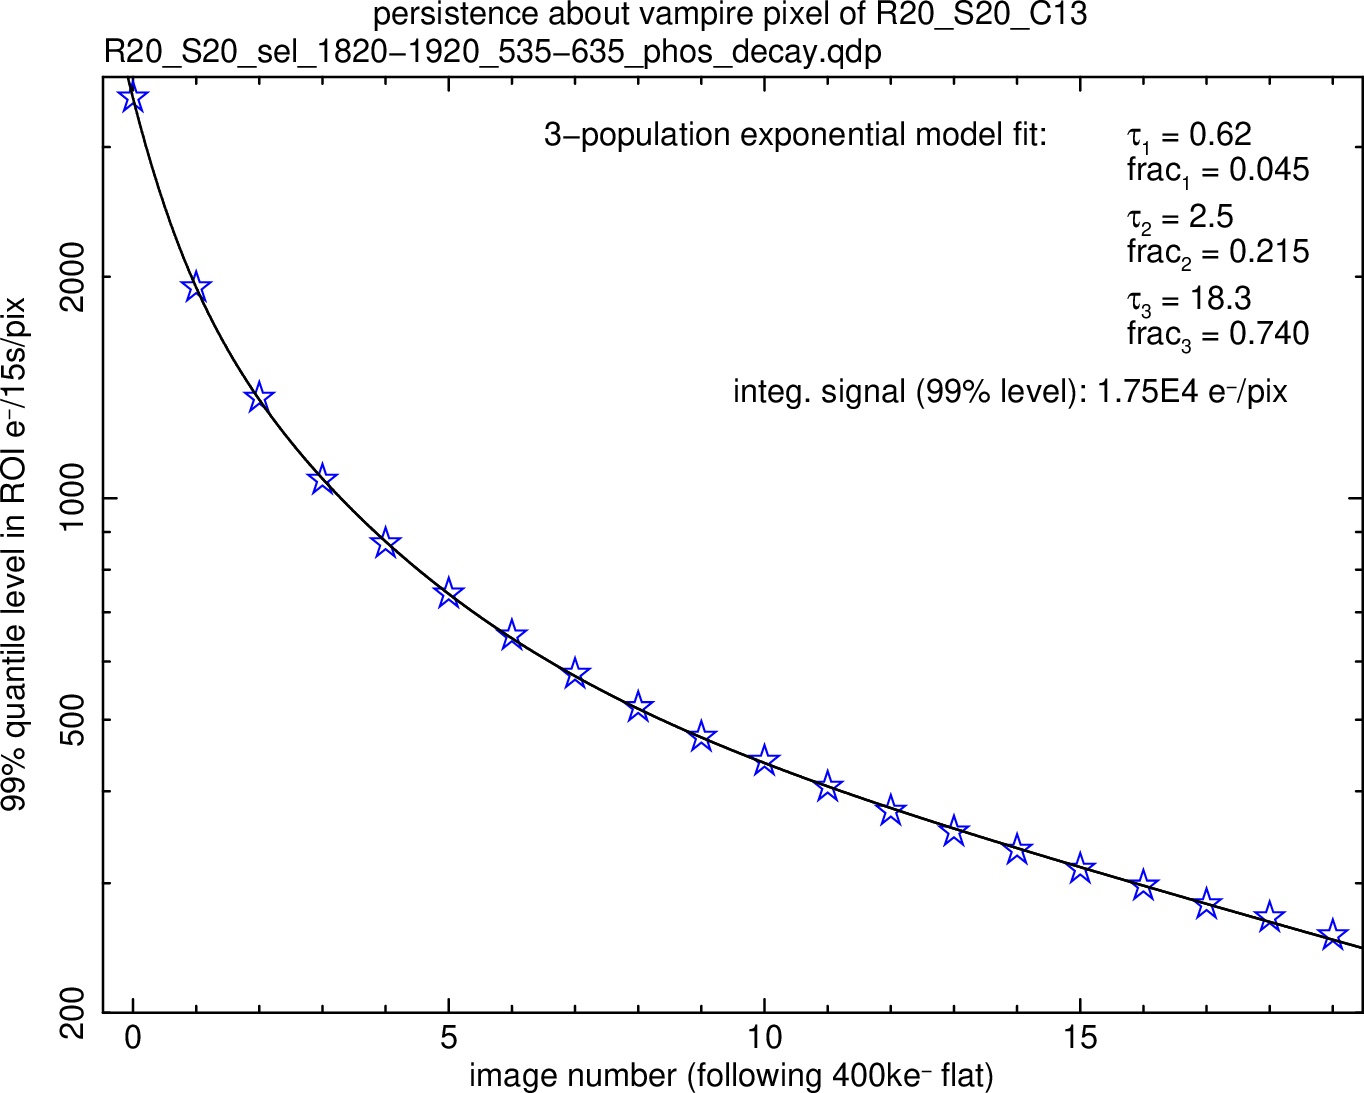
\includegraphics[width=\textwidth]{figures/phosphorescence-survey/phos_kinetics/R20_S20_sel_1820-1920_535-635_phos_decay_fit.png}    
\end{subfigure}
\caption{A three-population fit of the phosphorescence expressed by the vapire pixel region of R20\_S20\_C13. The fit was performed on the 99\% quantile level where signal levels are well above the $3\sigma$ level of the noise distribution. Here, image numbers are parasitically used as time units, with roughly 17.5 seconds per image.}
\label{fig:phos:kinetics:fit:R20S20C13}
\end{figure}

\begin{figure}[!htbp]
\begin{subfigure}{0.45\textwidth}    
  \centering
  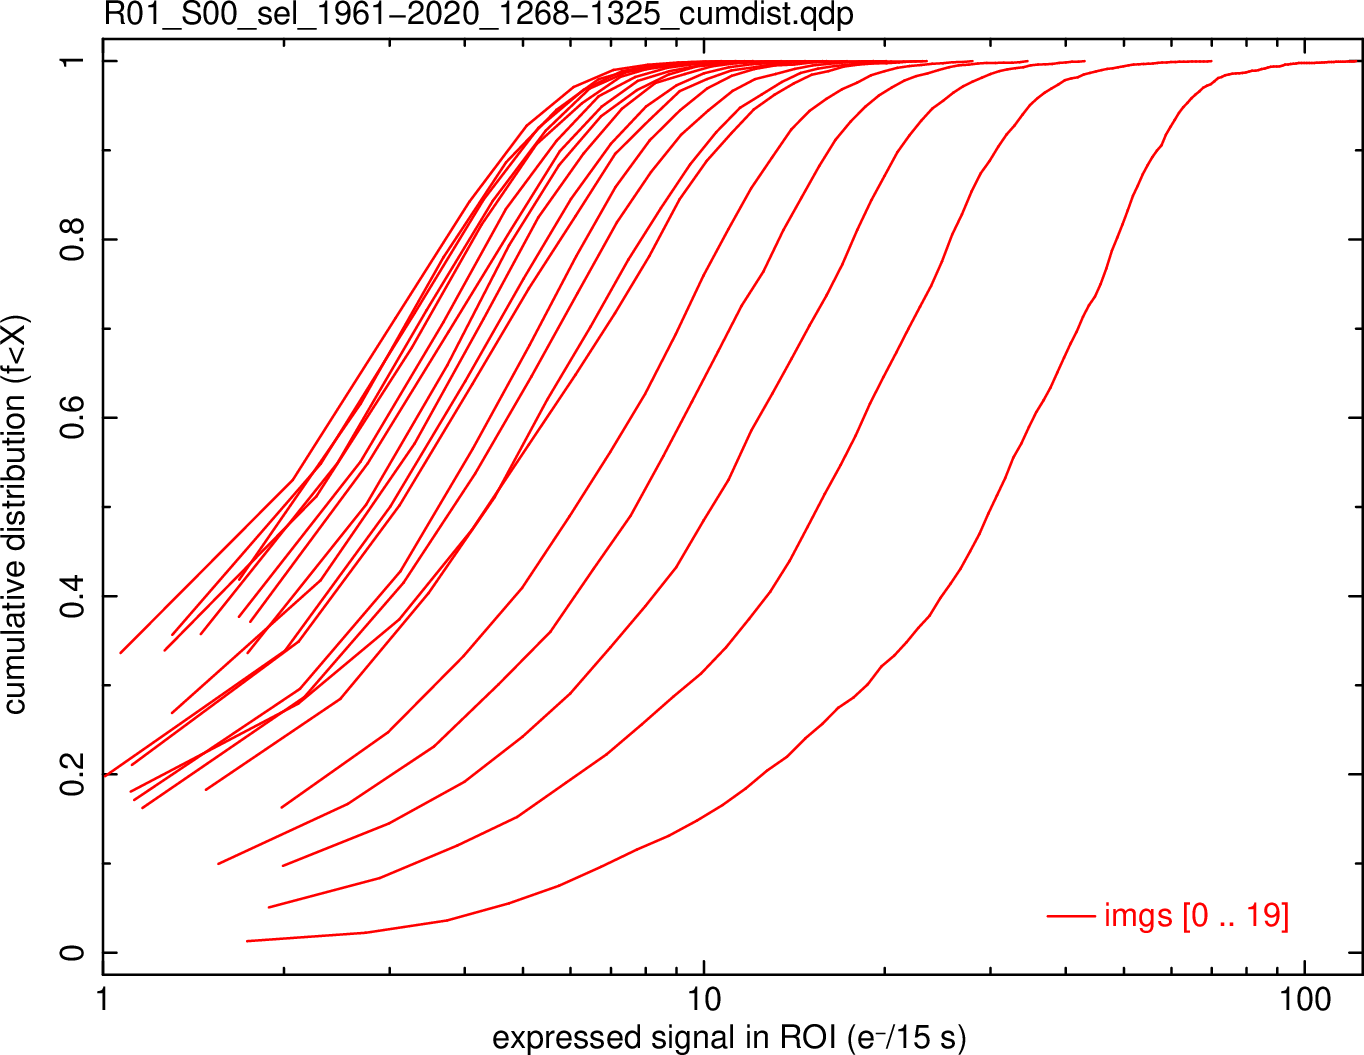
\includegraphics[width=\textwidth]{figures/phosphorescence-survey/phos_kinetics/R01_S00_sel_1961-2020_1268-1325_cumdist.png}    
\end{subfigure}
\hfil
\begin{subfigure}{0.45\textwidth}
  \centering
  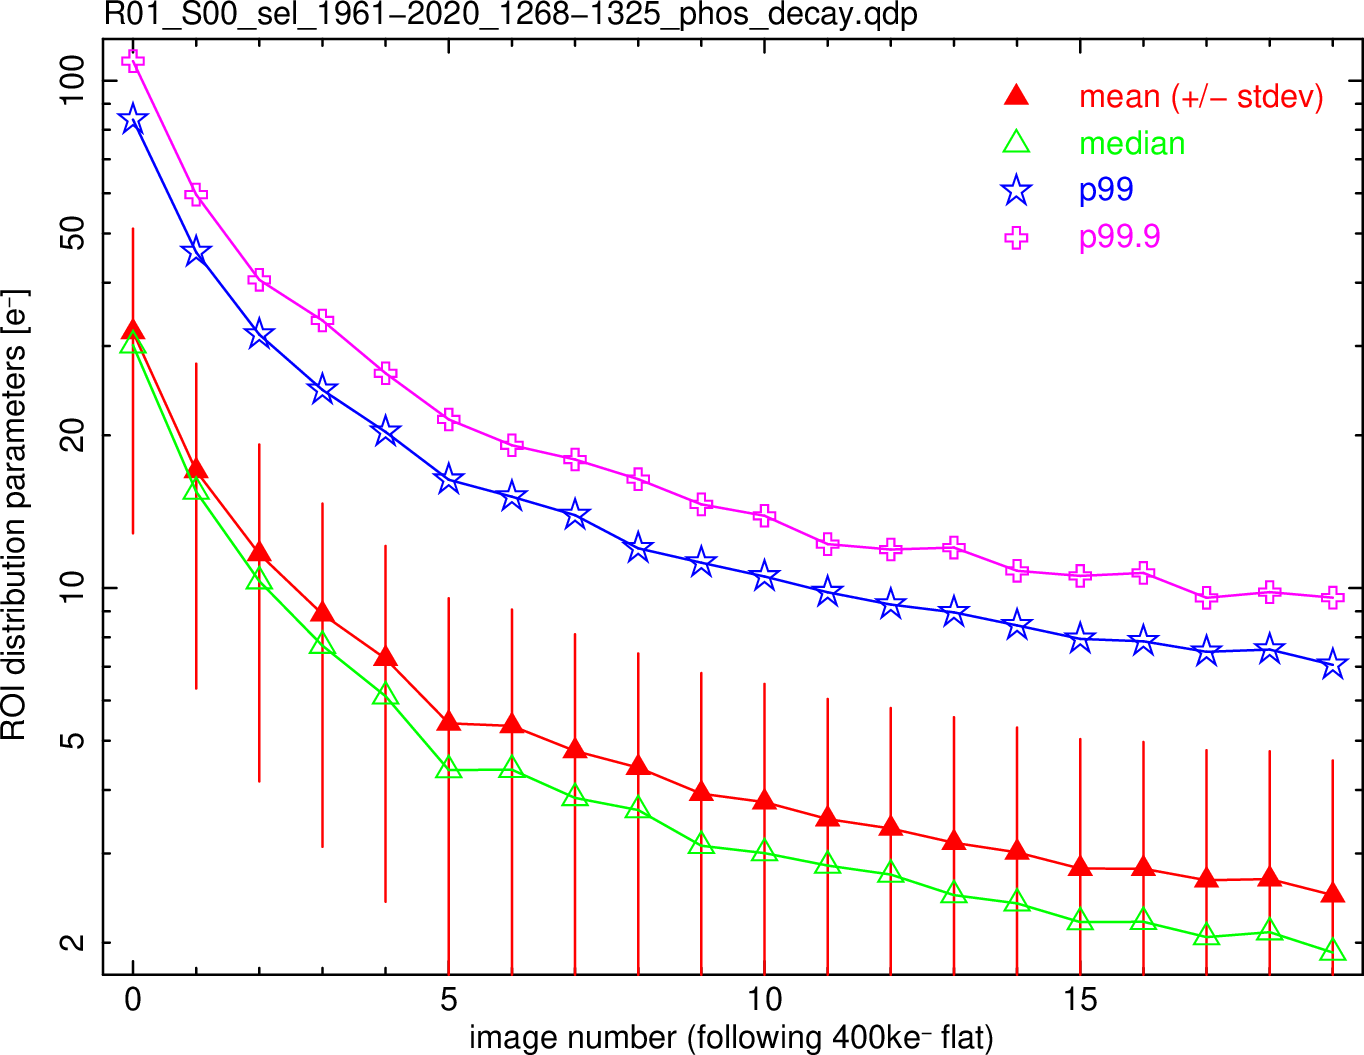
\includegraphics[width=\textwidth]{figures/phosphorescence-survey/phos_kinetics/R01_S00_sel_1961-2020_1268-1325_phos_decay.png}
\end{subfigure}
\newline
\begin{subfigure}{0.45\textwidth}    
  \centering
  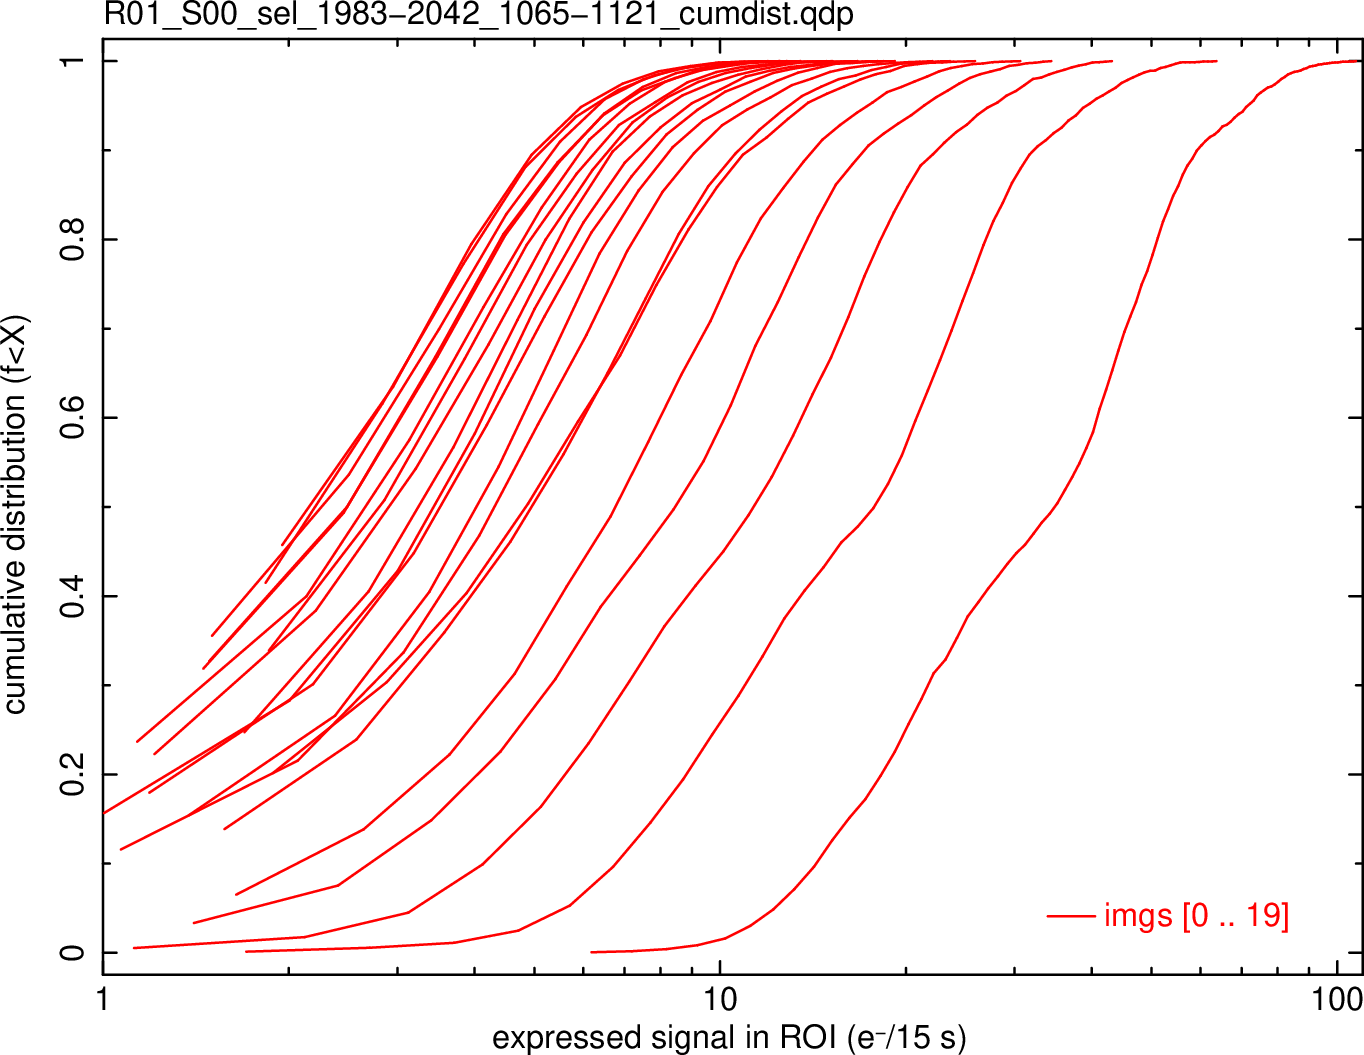
\includegraphics[width=\textwidth]{figures/phosphorescence-survey/phos_kinetics/R01_S00_sel_1983-2042_1065-1121_cumdist.png}    
\end{subfigure}
\hfil
\begin{subfigure}{0.45\textwidth}
  \centering
  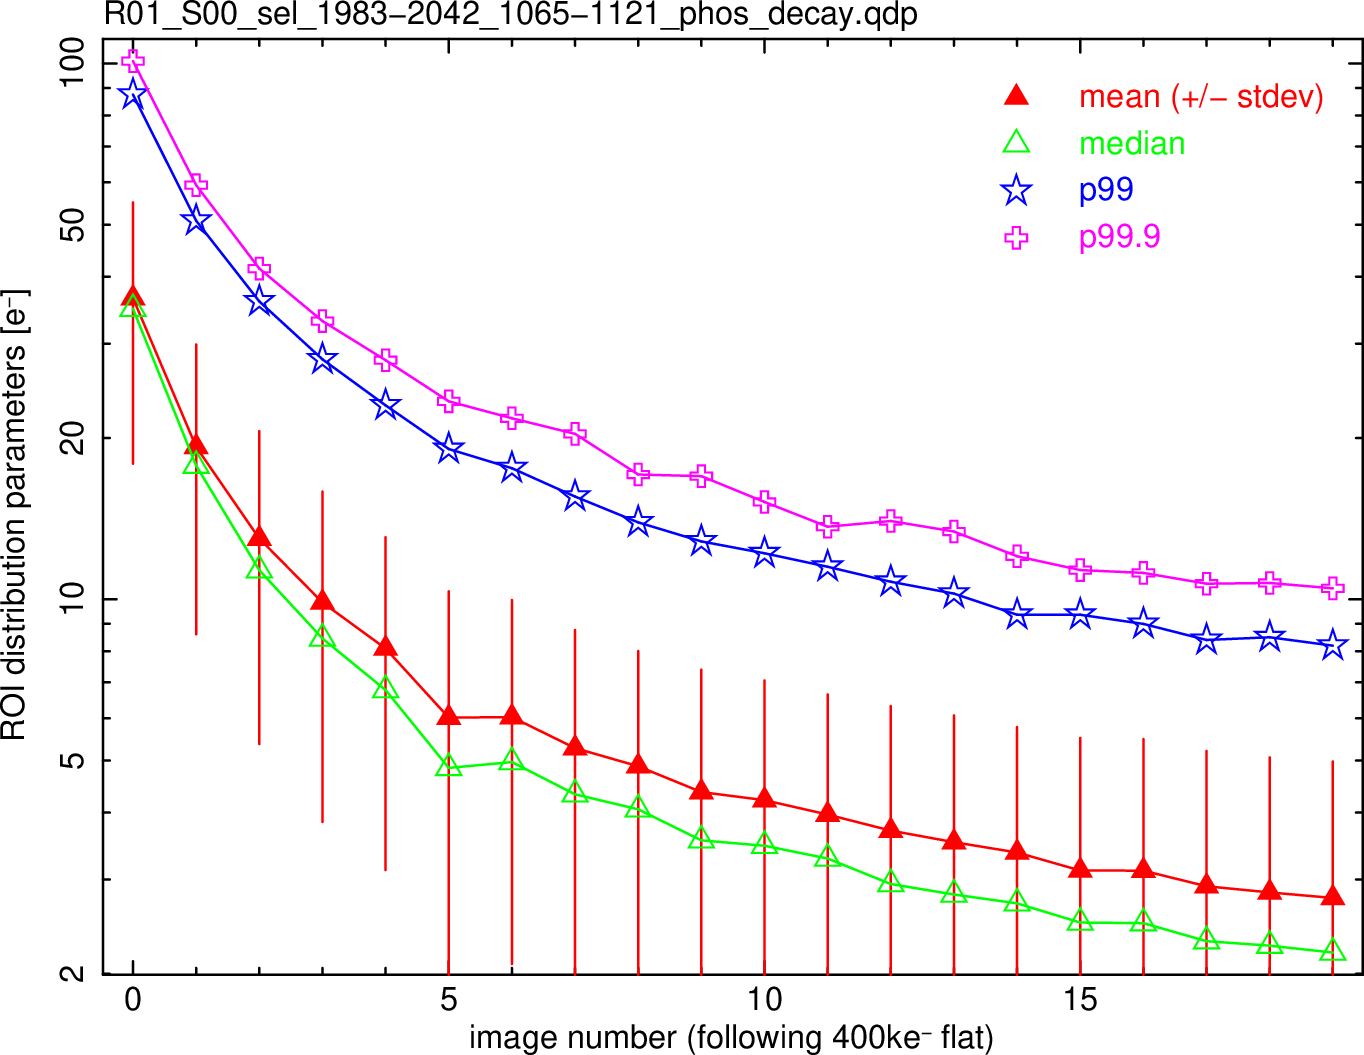
\includegraphics[width=\textwidth]{figures/phosphorescence-survey/phos_kinetics/R01_S00_sel_1983-2042_1065-1121_phos_decay.png}
\end{subfigure}
\newline
\begin{subfigure}{0.45\textwidth}    
  \centering
  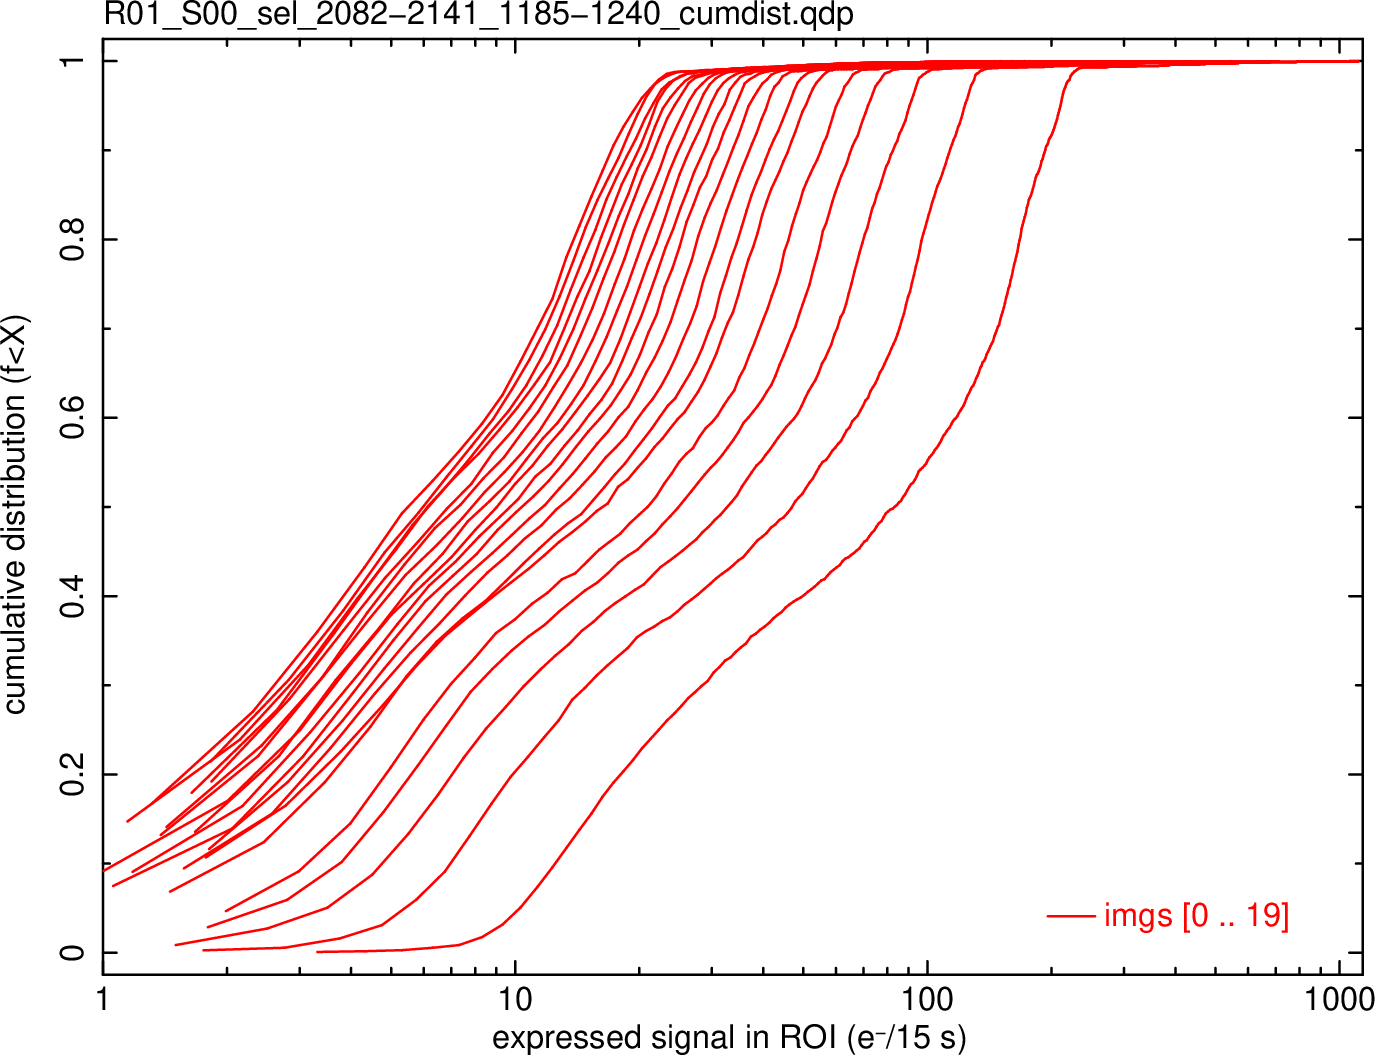
\includegraphics[width=\textwidth]{figures/phosphorescence-survey/phos_kinetics/R01_S00_sel_2082-2141_1185-1240_cumdist.png}    
\end{subfigure}
\hfil
\begin{subfigure}{0.45\textwidth}
  \centering
  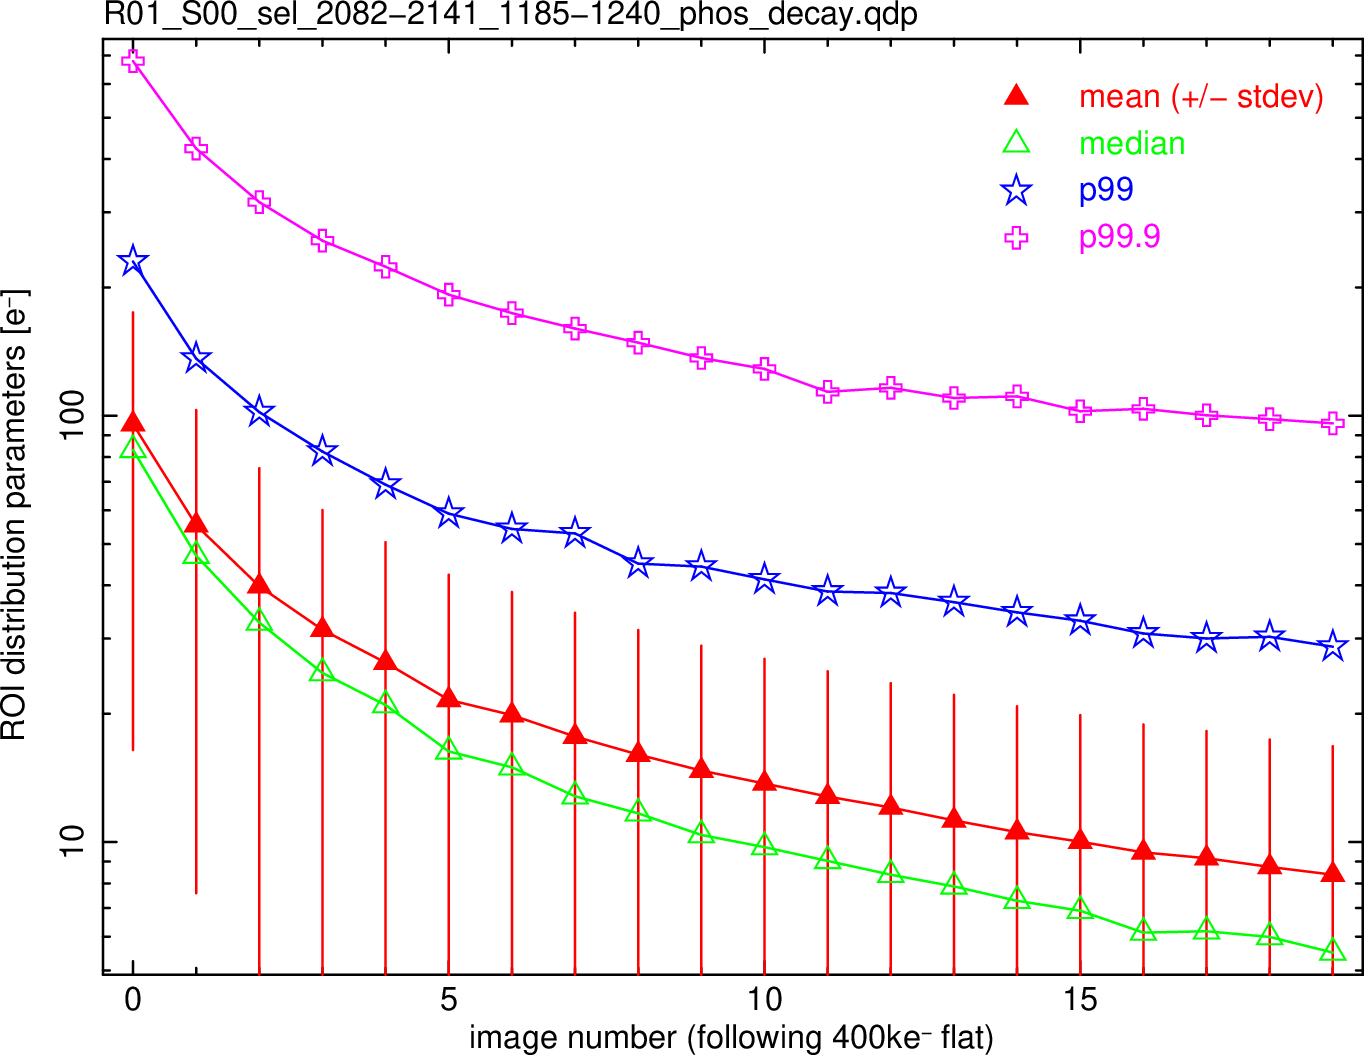
\includegraphics[width=\textwidth]{figures/phosphorescence-survey/phos_kinetics/R01_S00_sel_2082-2141_1185-1240_phos_decay.png}
\end{subfigure}
\newline
\caption{Kinetics for phosphorescence expression in ROIs of images for R01\_S00. This is the prominent cosmetic seen in Fig.~\ref{fig:phos:stains:R01S00}, which is apparently a {\it vampire} pixel.}
\label{fig:phos:kinetics:R01S00}
\end{figure}

\begin{figure}[!htbp]
\begin{subfigure}{0.45\textwidth}    
  \centering
  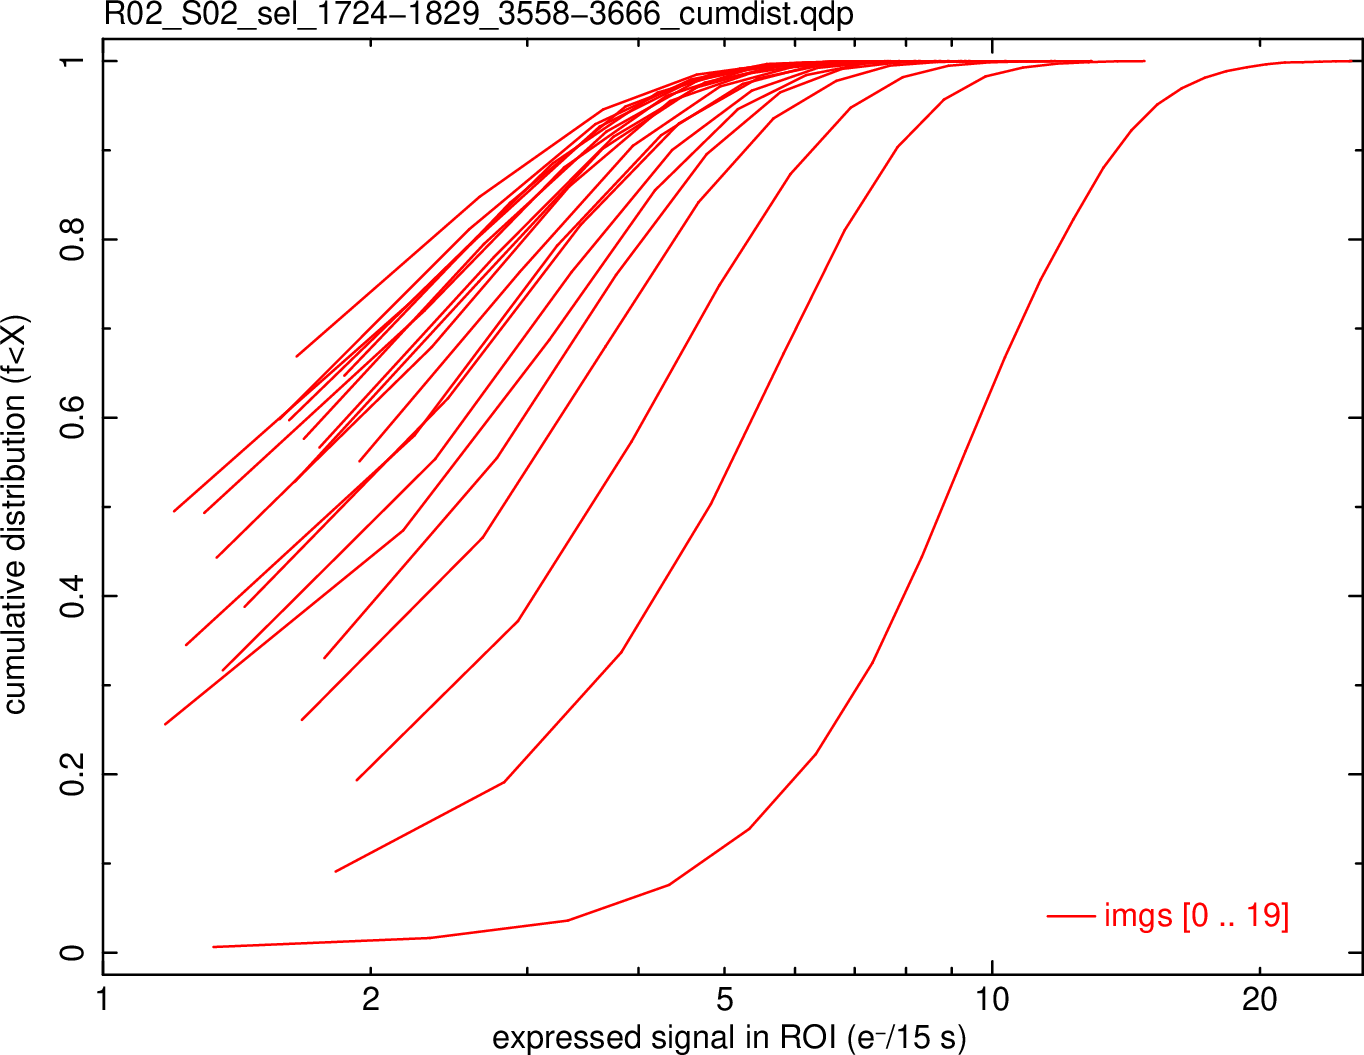
\includegraphics[width=\textwidth]{figures/phosphorescence-survey/phos_kinetics/R02_S02_sel_1724-1829_3558-3666_cumdist.png}    
\end{subfigure}
\hfil
\begin{subfigure}{0.45\textwidth}
  \centering
  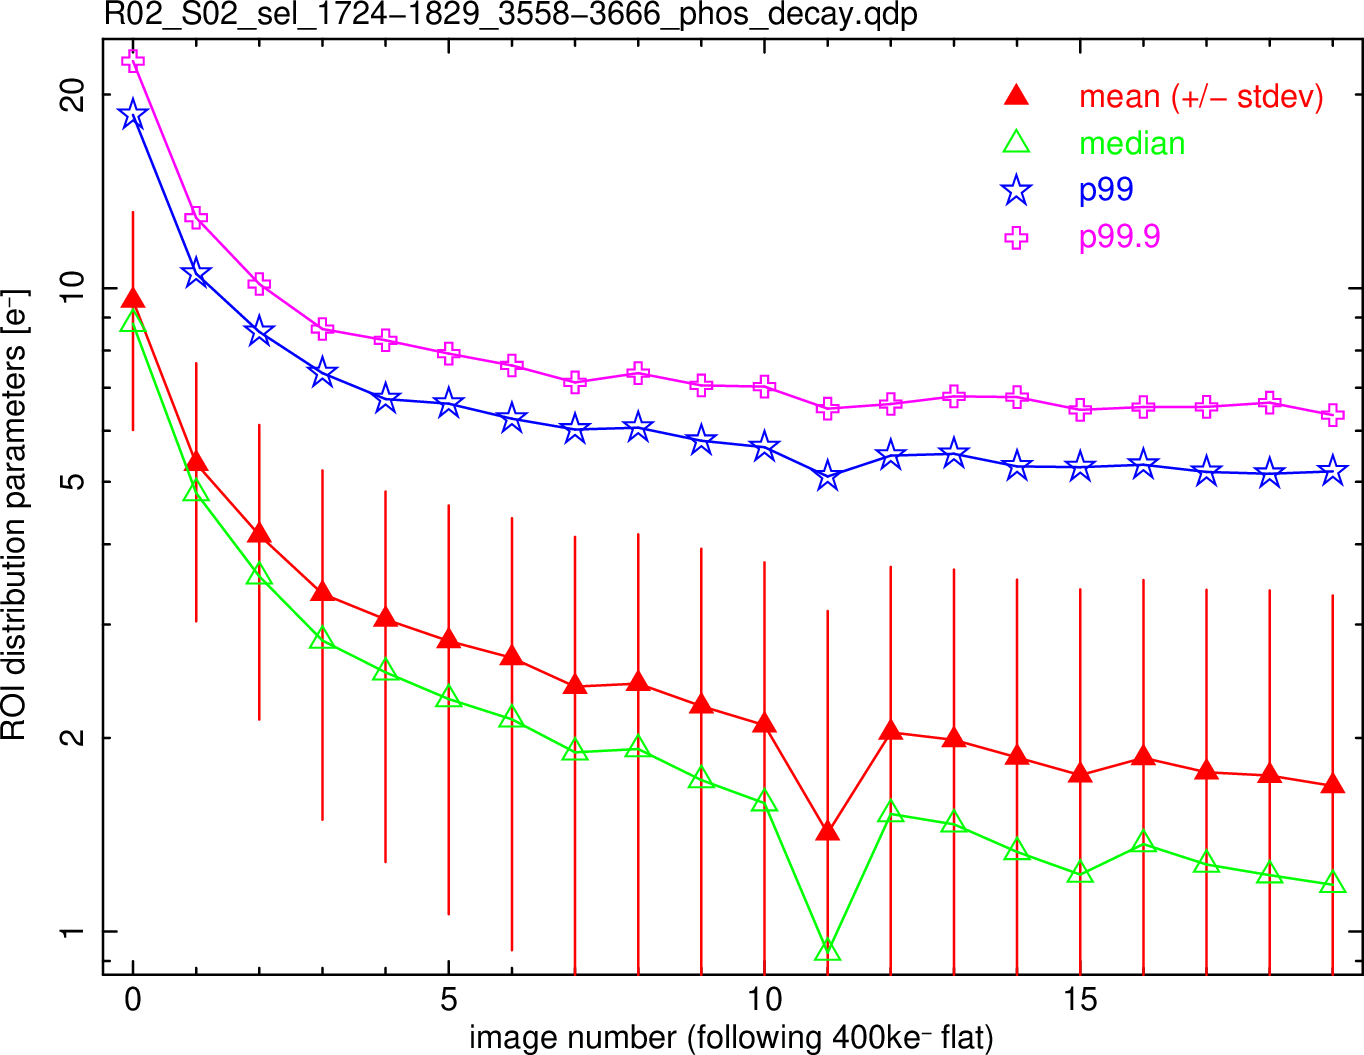
\includegraphics[width=\textwidth]{figures/phosphorescence-survey/phos_kinetics/R02_S02_sel_1724-1829_3558-3666_phos_decay.png}
\end{subfigure}
\newline
\begin{subfigure}{0.45\textwidth}    
  \centering
  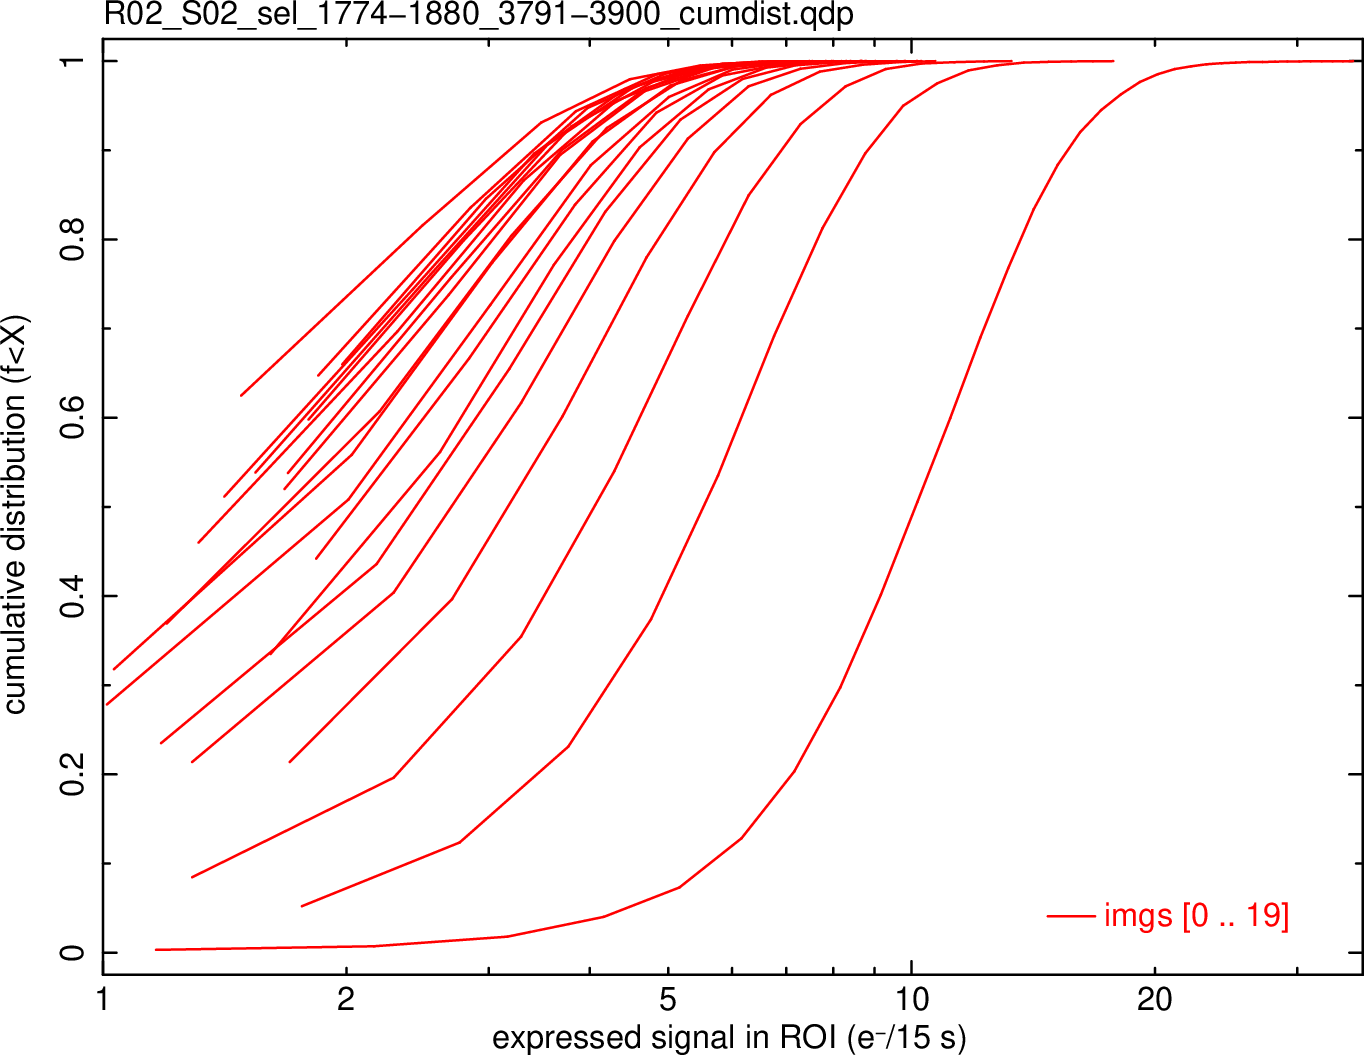
\includegraphics[width=\textwidth]{figures/phosphorescence-survey/phos_kinetics/R02_S02_sel_1774-1880_3791-3900_cumdist.png}    
\end{subfigure}
\hfil
\begin{subfigure}{0.45\textwidth}
  \centering
  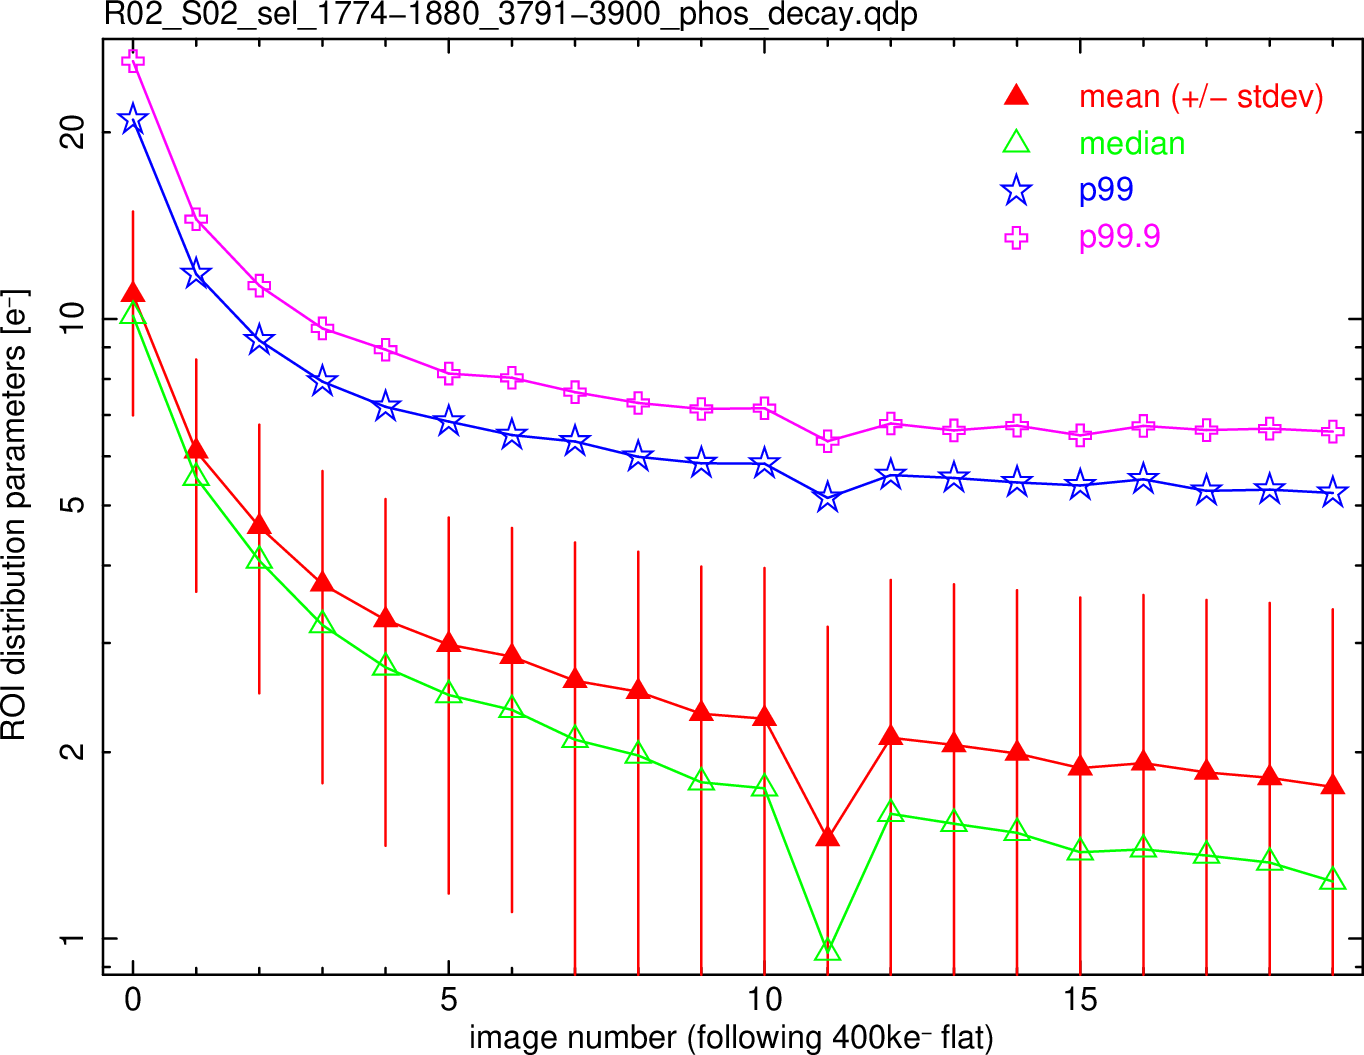
\includegraphics[width=\textwidth]{figures/phosphorescence-survey/phos_kinetics/R02_S02_sel_1774-1880_3791-3900_phos_decay.png}
\end{subfigure}
\newline
\begin{subfigure}{0.45\textwidth}    
  \centering
  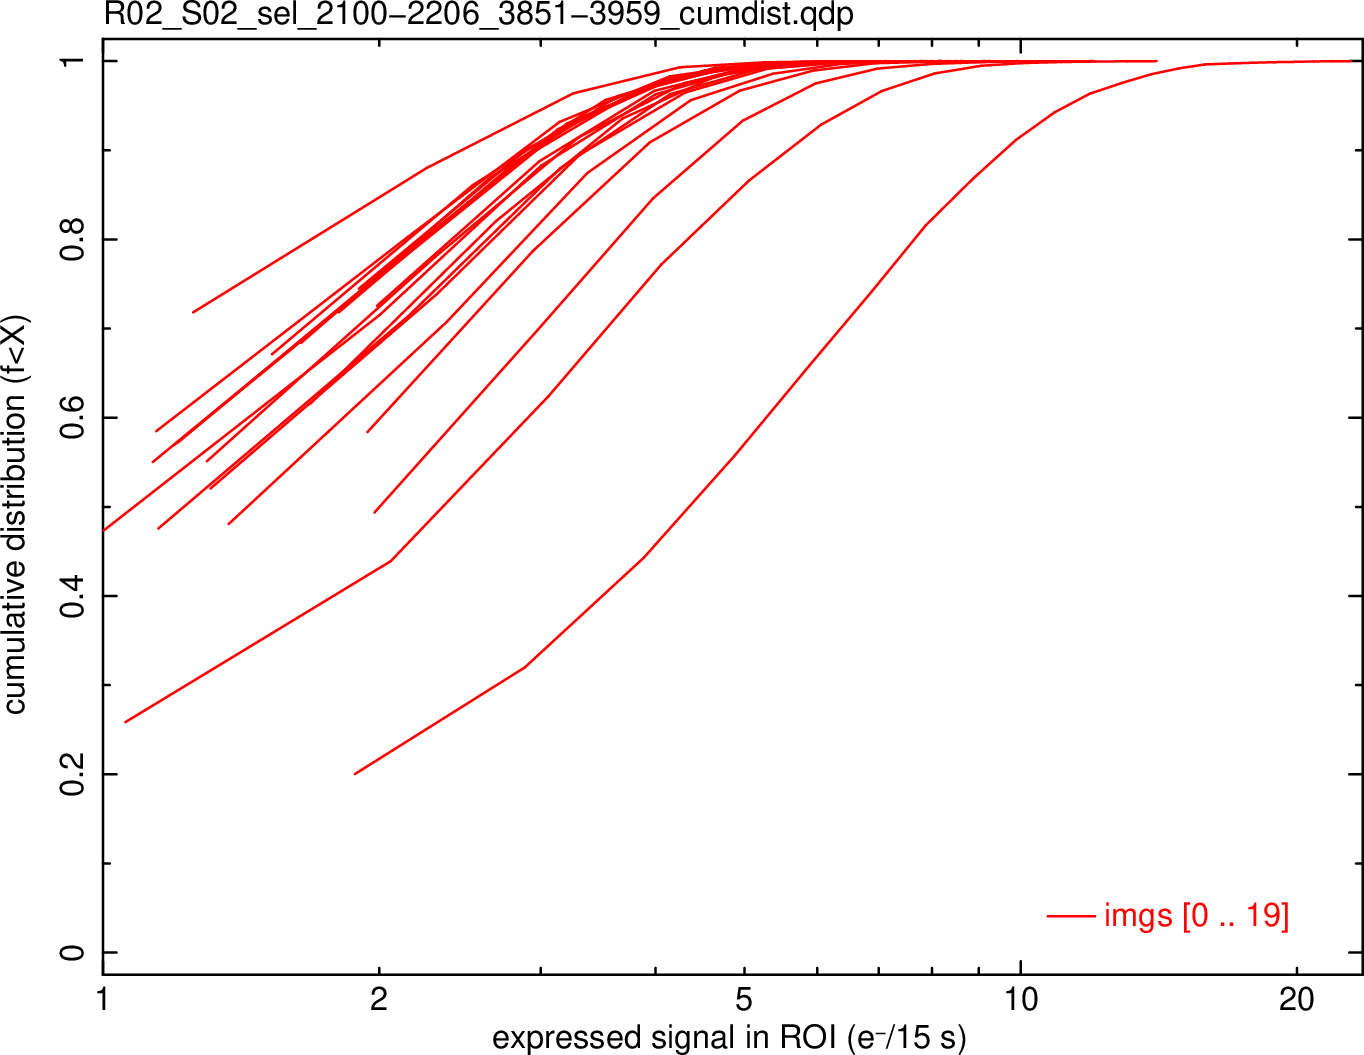
\includegraphics[width=\textwidth]{figures/phosphorescence-survey/phos_kinetics/R02_S02_sel_2100-2206_3851-3959_cumdist.png}    
\end{subfigure}
\hfil
\begin{subfigure}{0.45\textwidth}
  \centering
  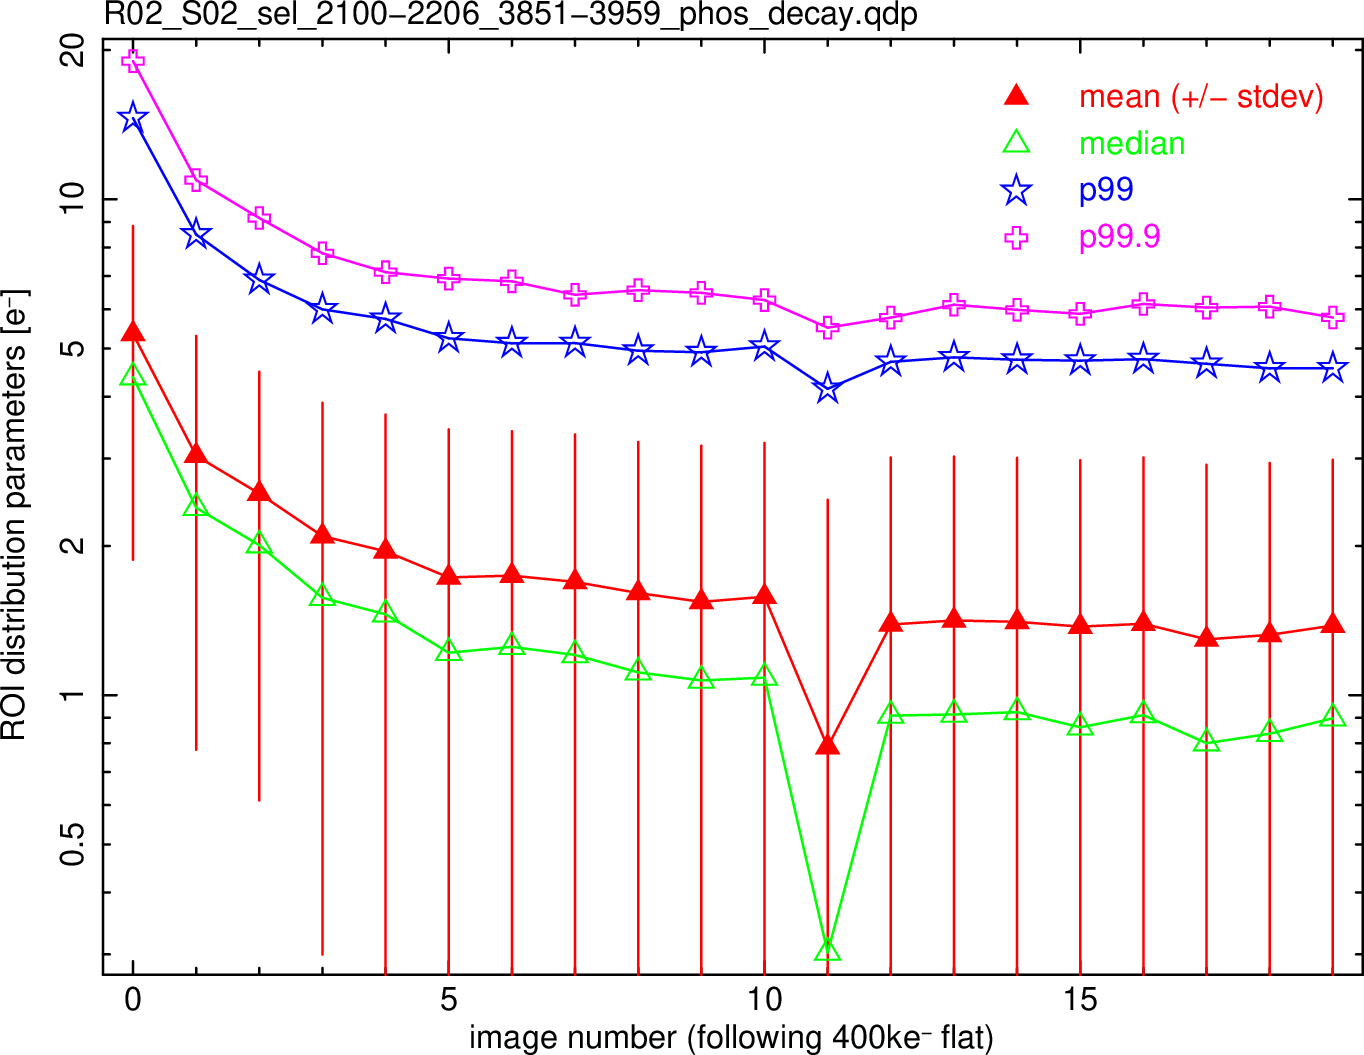
\includegraphics[width=\textwidth]{figures/phosphorescence-survey/phos_kinetics/R02_S02_sel_2100-2206_3851-3959_phos_decay.png}
\end{subfigure}
\newline
\caption{Kinetics for phosphorescence expression in ROIs of images for R02\_S02. This is the diffuse phosphorescence that correlates with the coffee stains seen in Fig.~\ref{fig:phos:stains:R02S02}. No extractions were performed on the {\it vampire pixels} found on the same sensor (R02\_S02\_C15 and R02\_S02\_C07).}
\label{fig:phos:kinetics:R02S02}
\end{figure}

\begin{figure}[!htbp]
\begin{subfigure}{0.45\textwidth}    
  \centering
  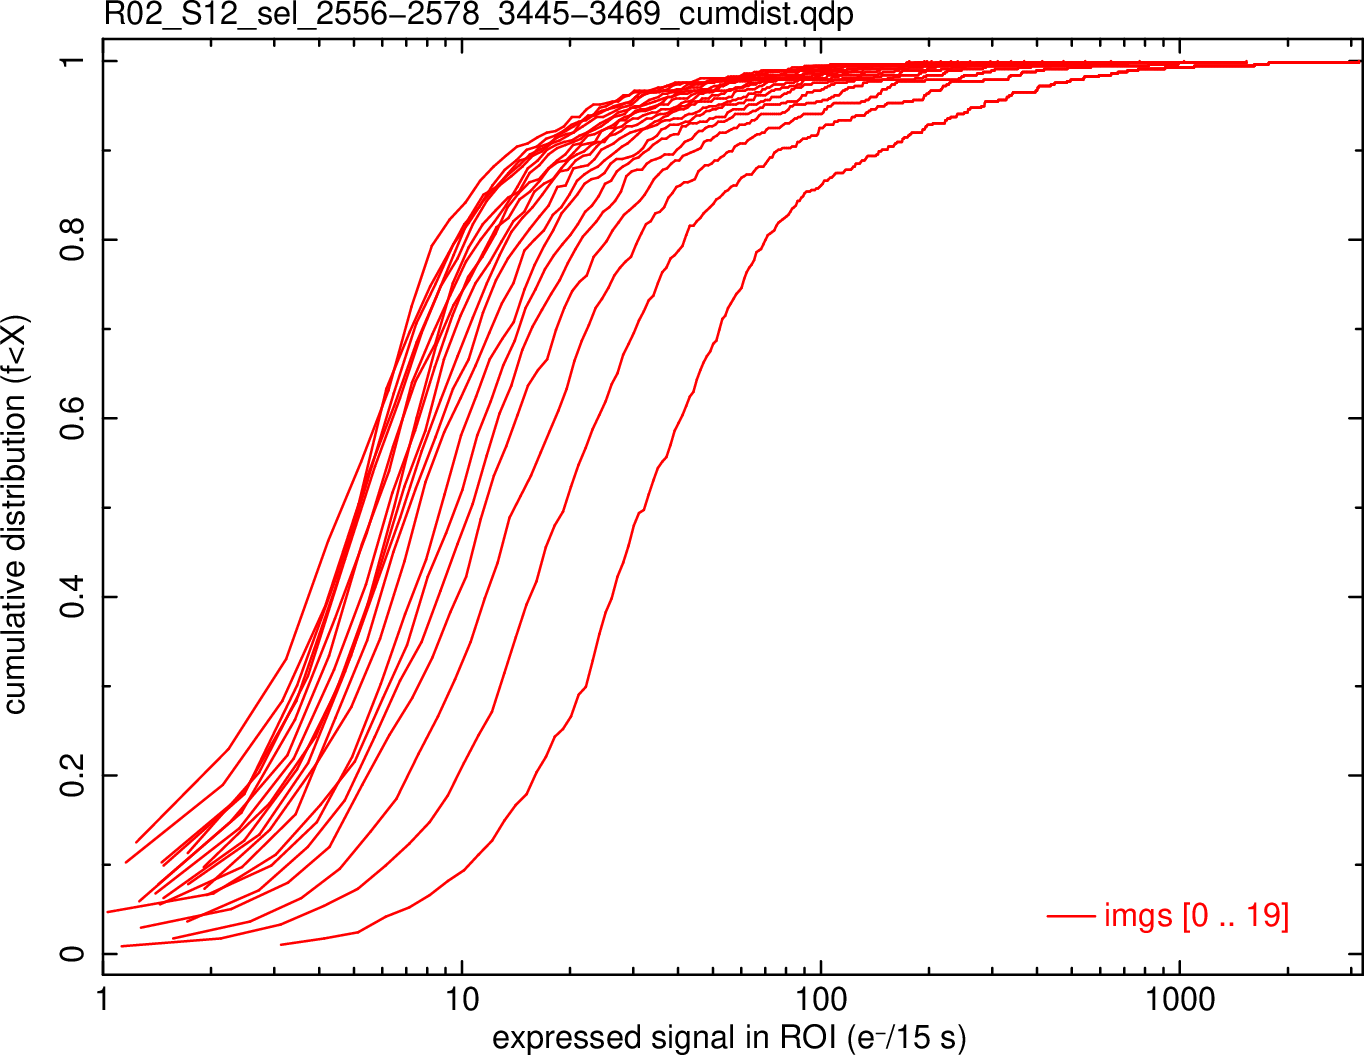
\includegraphics[width=\textwidth]{figures/phosphorescence-survey/phos_kinetics/R02_S12_sel_2556-2578_3445-3469_cumdist.png}    
\end{subfigure}
\hfil
\begin{subfigure}{0.45\textwidth}
  \centering
  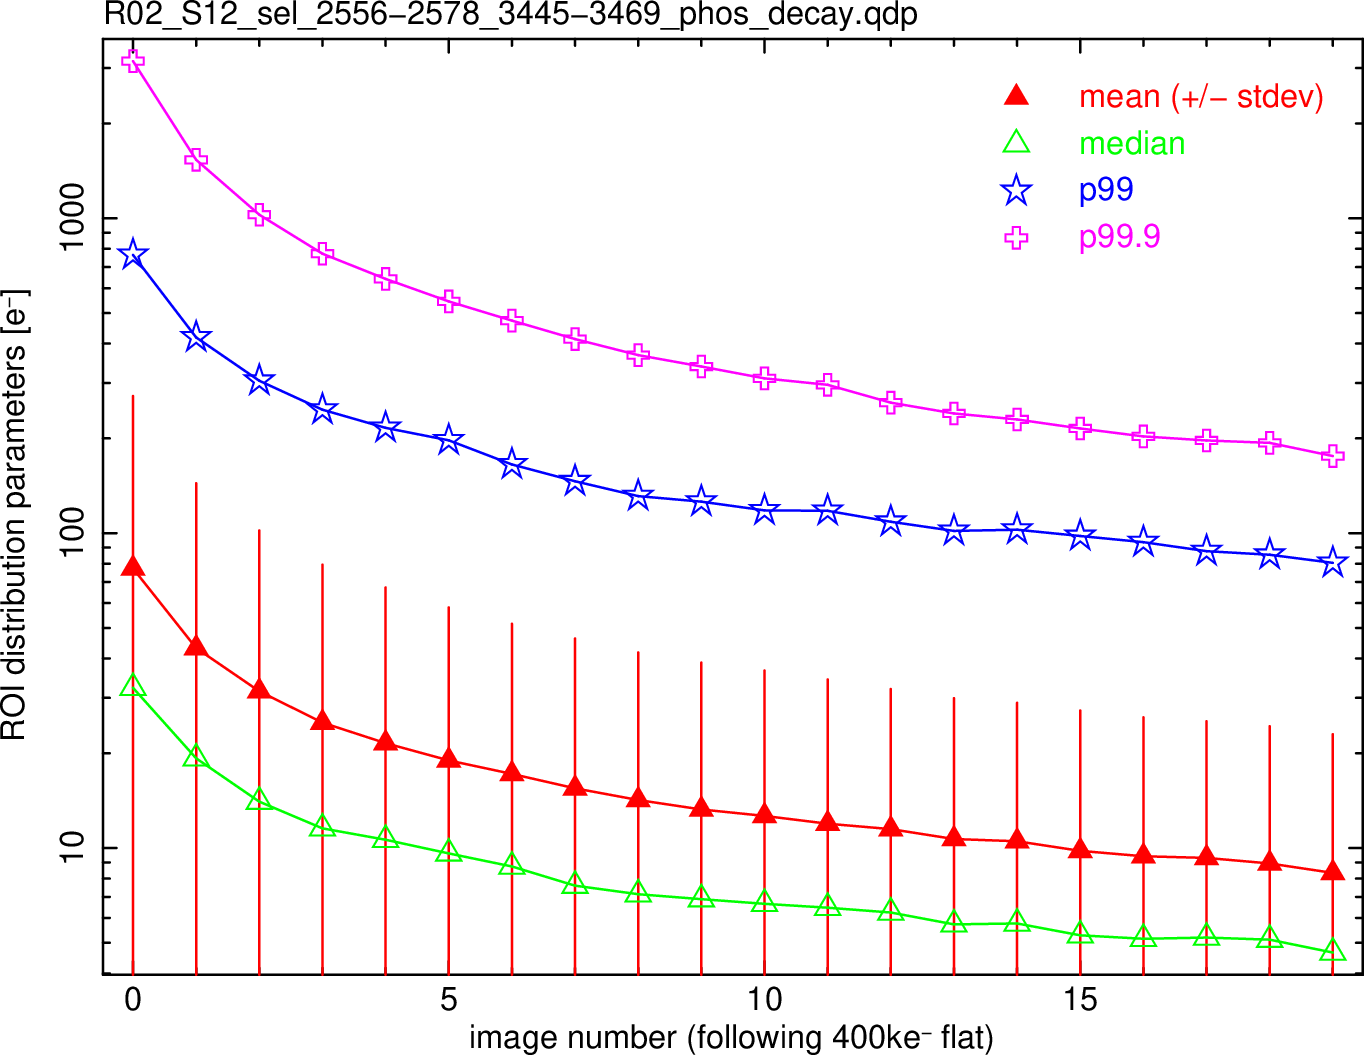
\includegraphics[width=\textwidth]{figures/phosphorescence-survey/phos_kinetics/R02_S12_sel_2556-2578_3445-3469_phos_decay.png}
\end{subfigure}
\newline
\begin{subfigure}{0.45\textwidth}    
  \centering
  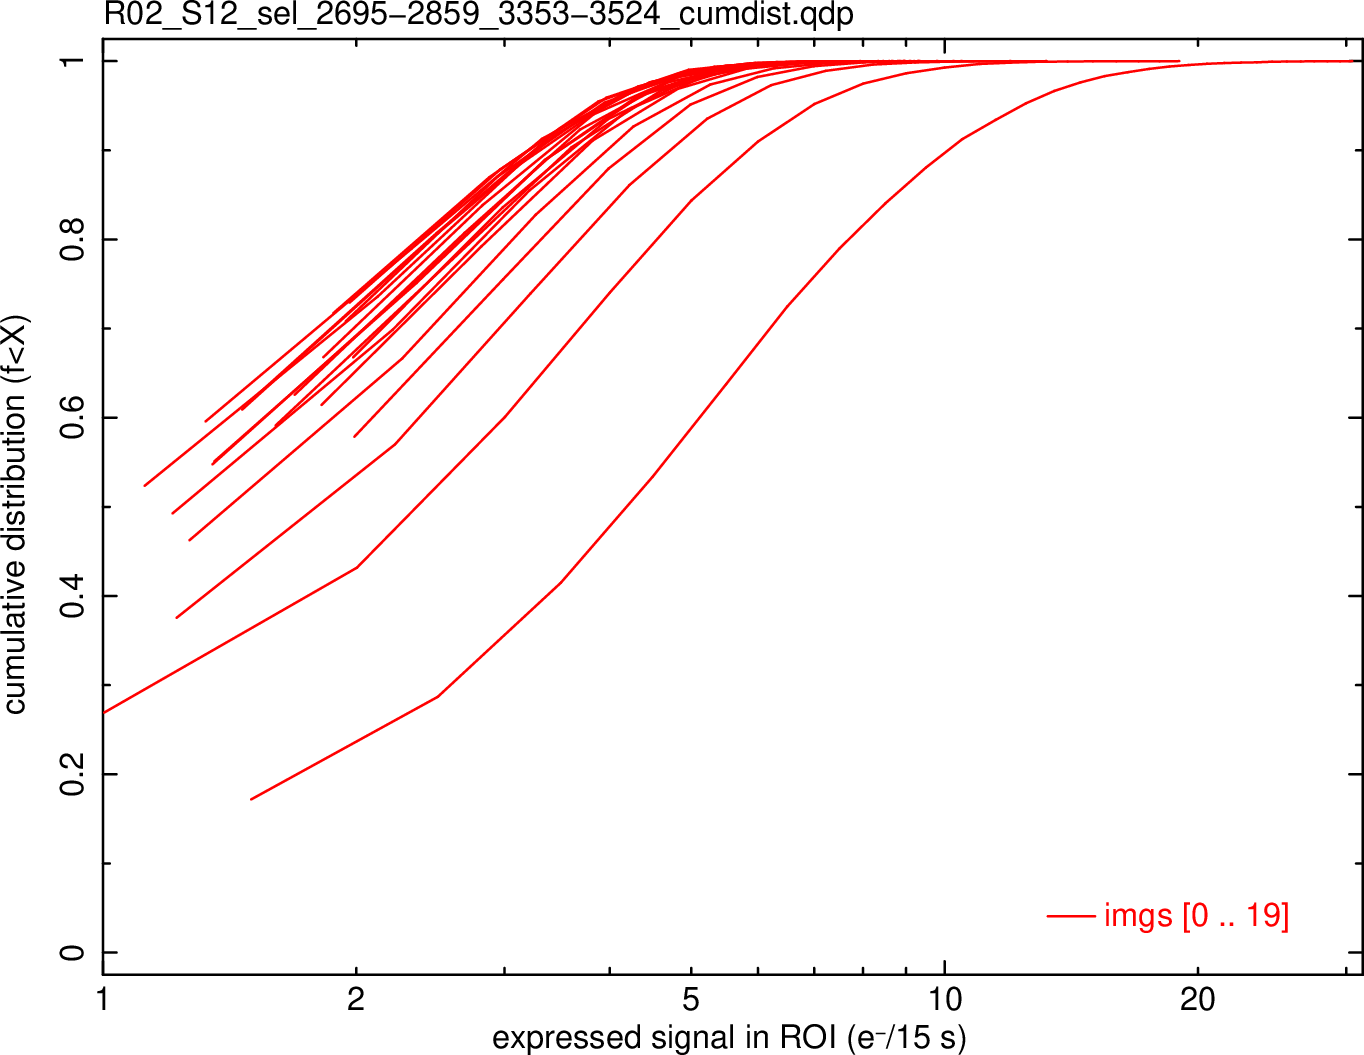
\includegraphics[width=\textwidth]{figures/phosphorescence-survey/phos_kinetics/R02_S12_sel_2695-2859_3353-3524_cumdist.png}    
\end{subfigure}
\hfil
\begin{subfigure}{0.45\textwidth}
  \centering
  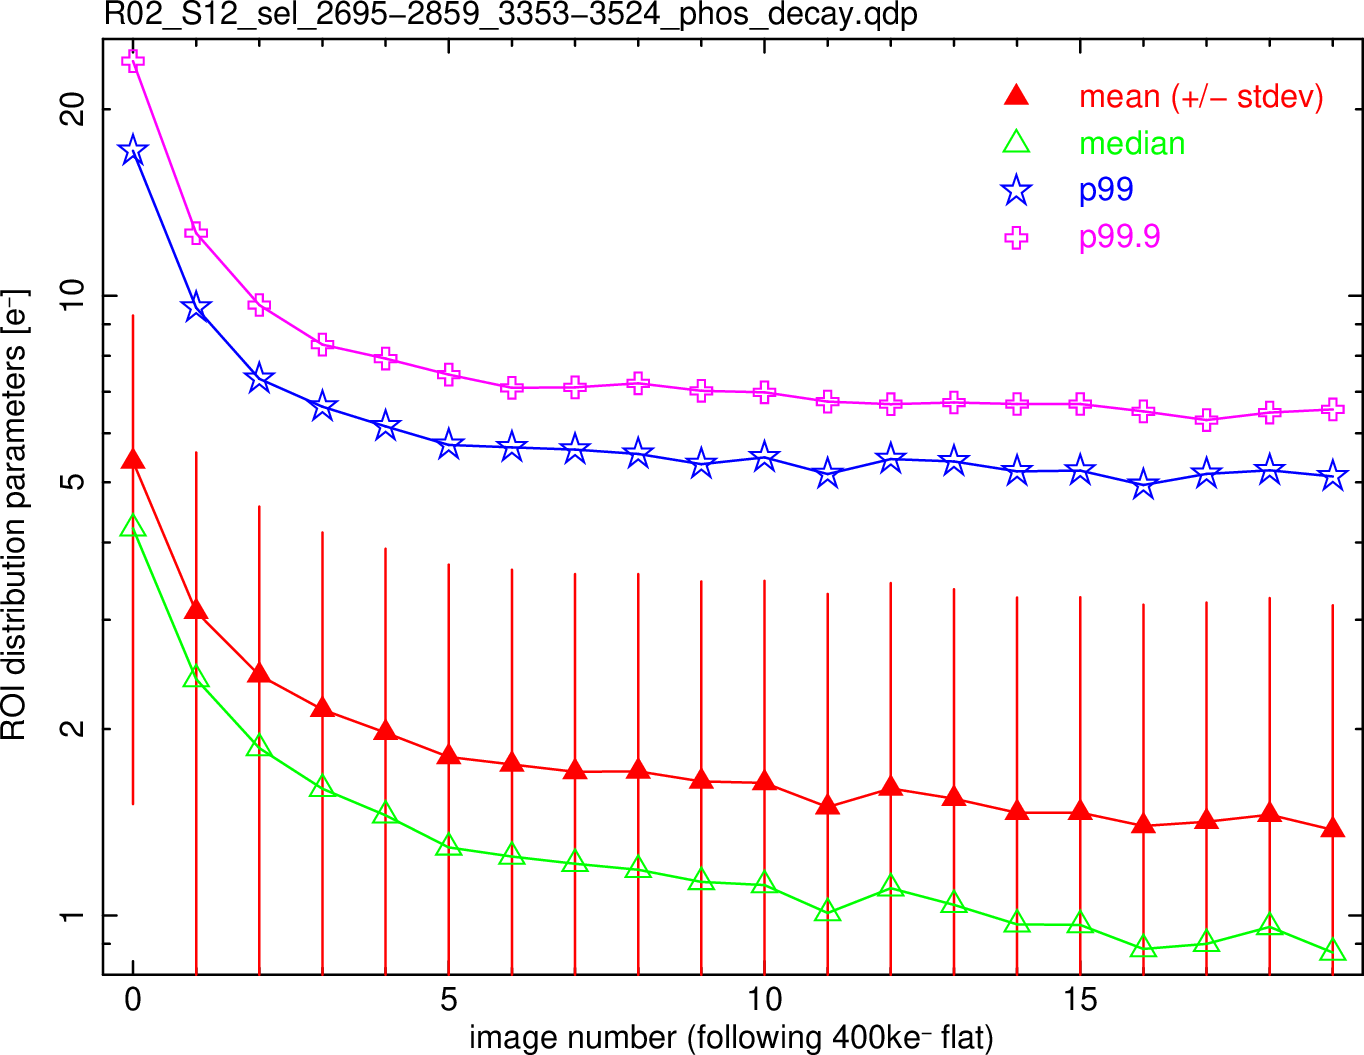
\includegraphics[width=\textwidth]{figures/phosphorescence-survey/phos_kinetics/R02_S12_sel_2695-2859_3353-3524_phos_decay.png}
\end{subfigure}
\newline
\begin{subfigure}{0.45\textwidth}    
  \centering
  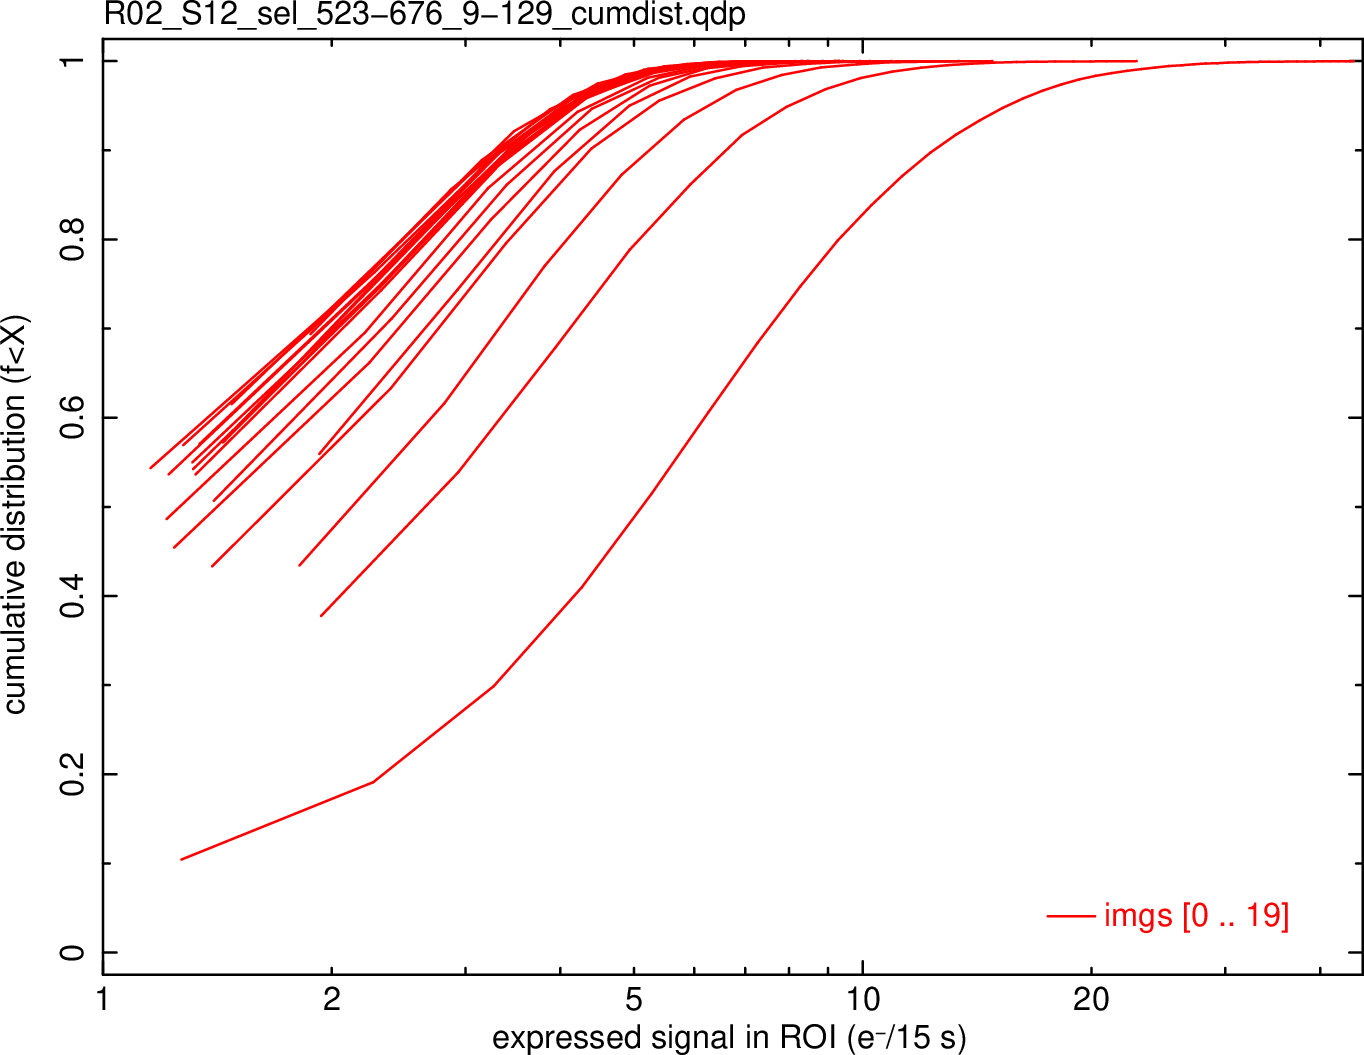
\includegraphics[width=\textwidth]{figures/phosphorescence-survey/phos_kinetics/R02_S12_sel_523-676_9-129_cumdist.png}    
\end{subfigure}
\hfil
\begin{subfigure}{0.45\textwidth}
  \centering
  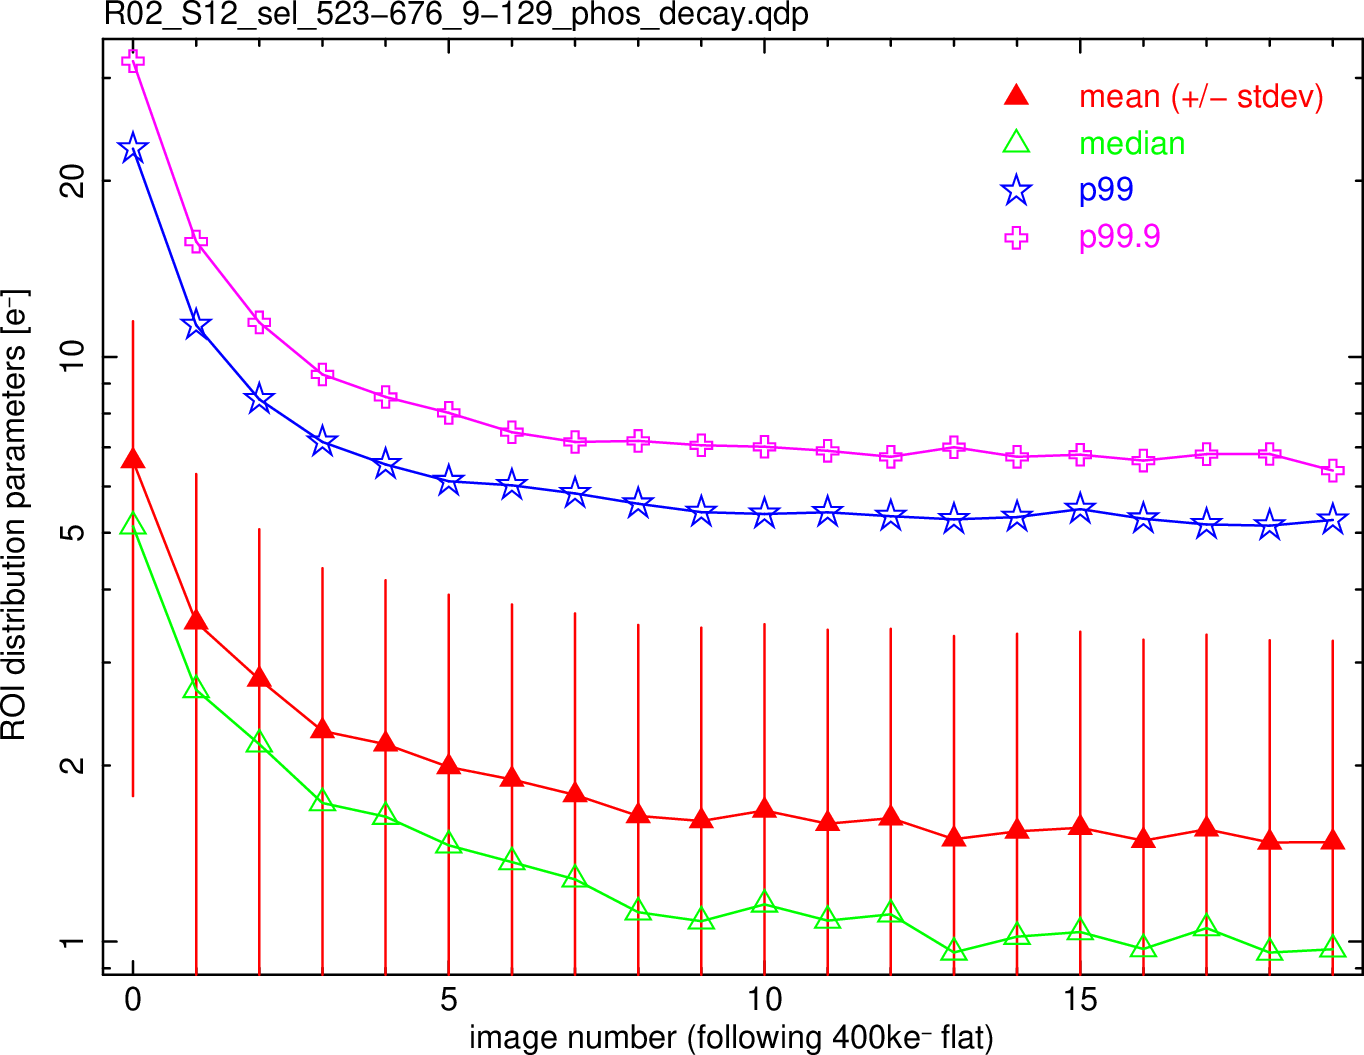
\includegraphics[width=\textwidth]{figures/phosphorescence-survey/phos_kinetics/R02_S12_sel_523-676_9-129_phos_decay.png}
\end{subfigure}
\newline
\caption{Kinetics for phosphorescence expression in ROIs of images for R02\_S12. This is the structured phosphorescence that correlates with the coffee stains seen in Fig.~\ref{fig:phos:stains:R02S12}.}
\label{fig:phos:kinetics:R02S12}
\end{figure}

\begin{figure}[!htbp]
\begin{subfigure}{0.45\textwidth}    
  \centering
  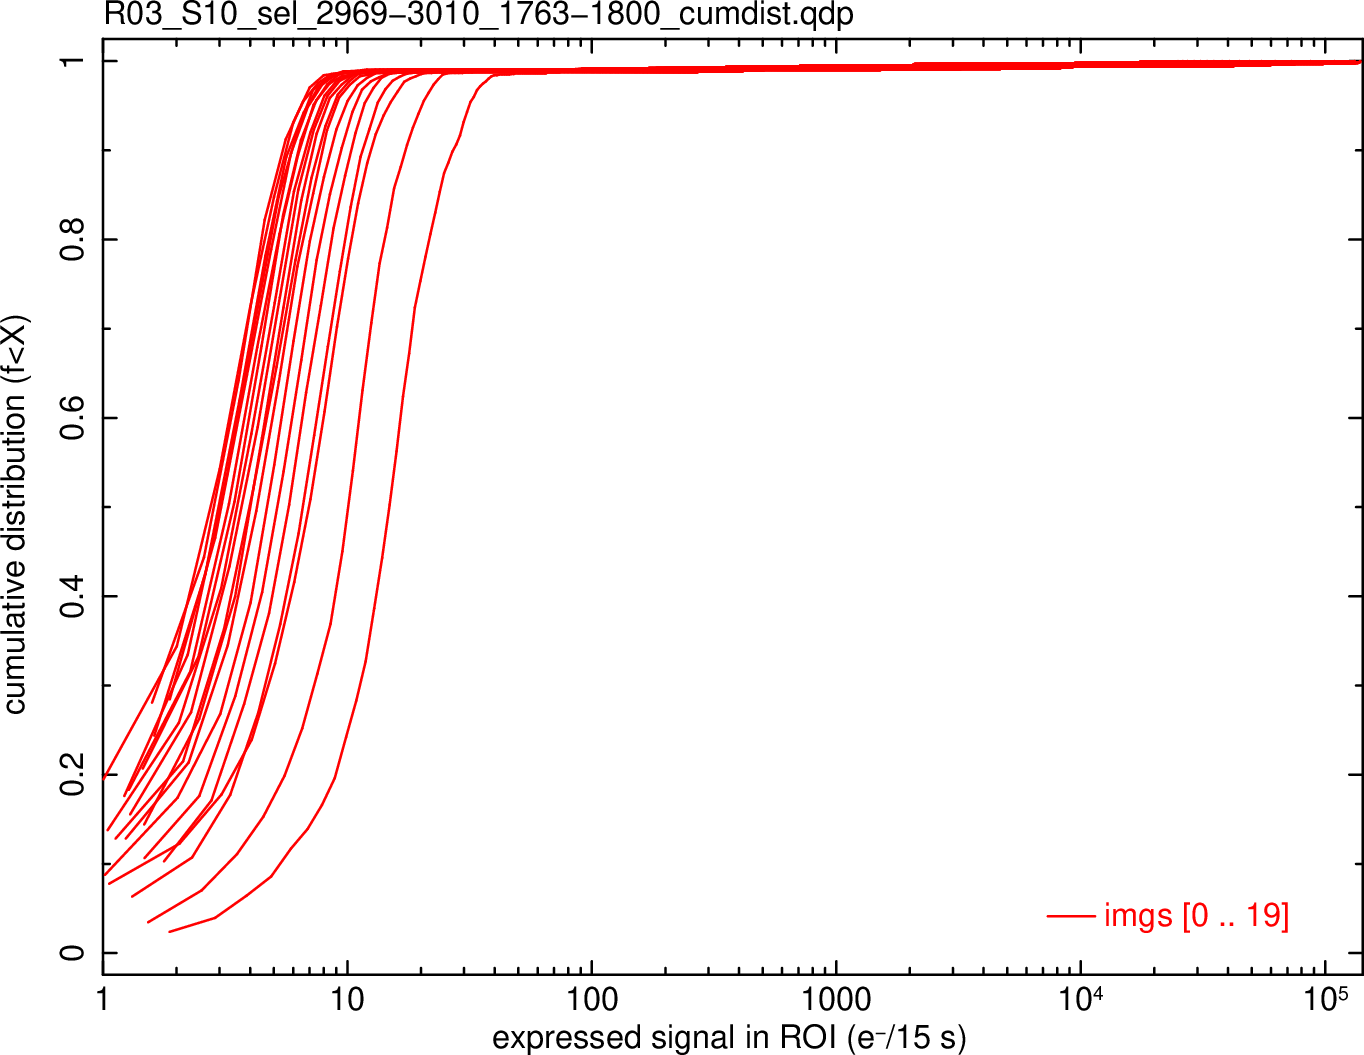
\includegraphics[width=\textwidth]{figures/phosphorescence-survey/phos_kinetics/R03_S10_sel_2969-3010_1763-1800_cumdist.png}    
\end{subfigure}
\hfil
\begin{subfigure}{0.45\textwidth}
  \centering
  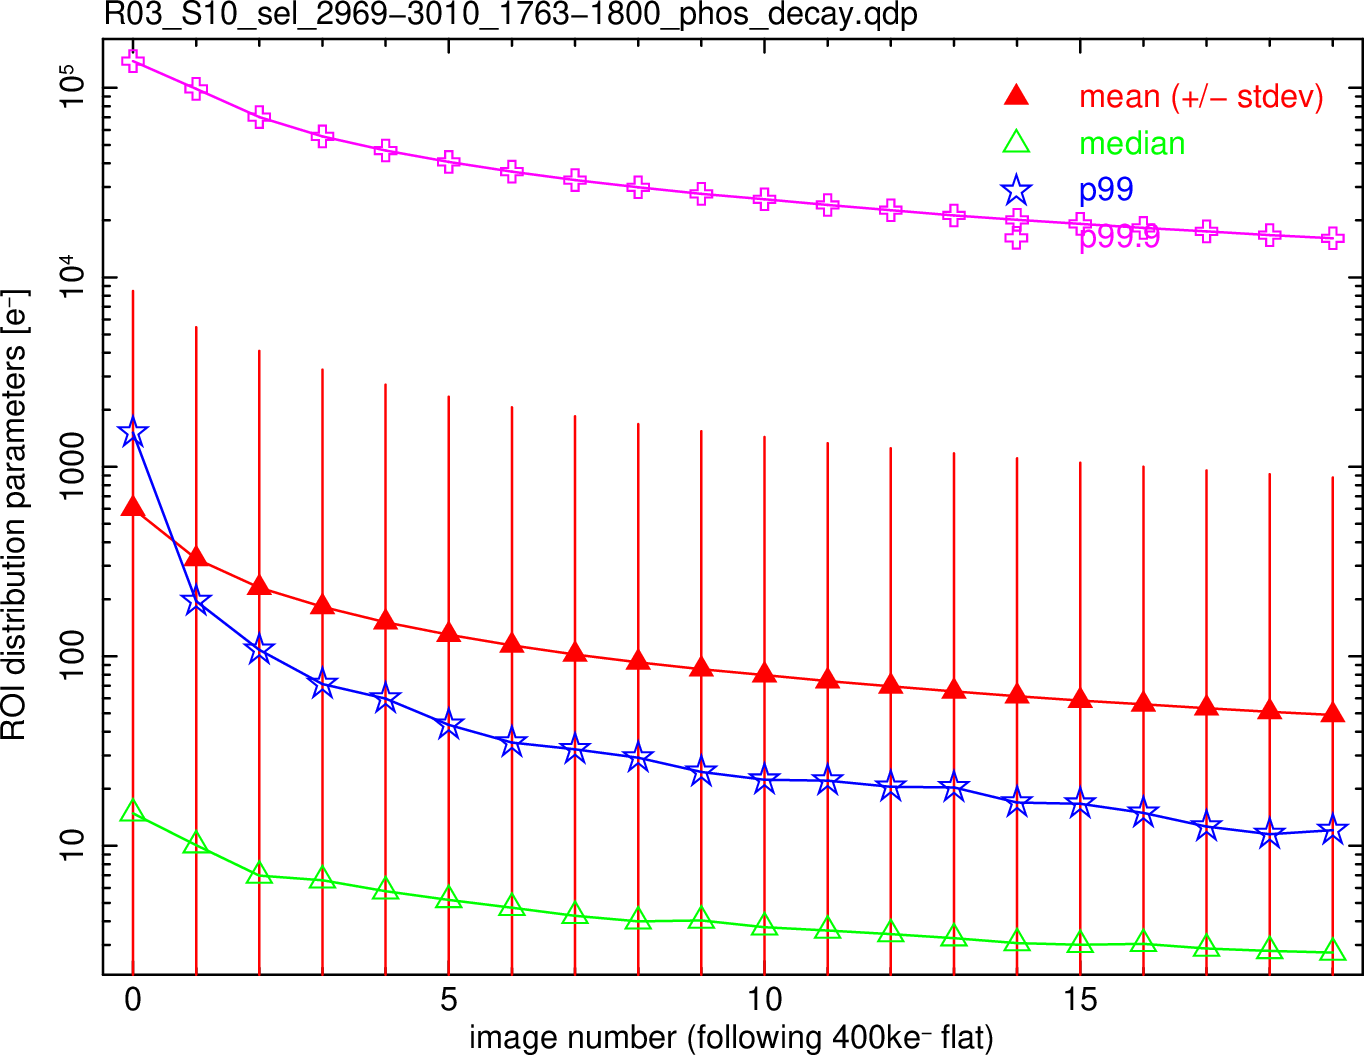
\includegraphics[width=\textwidth]{figures/phosphorescence-survey/phos_kinetics/R03_S10_sel_2969-3010_1763-1800_phos_decay.png}
\end{subfigure}
\newline
\begin{subfigure}{0.45\textwidth}    
  \centering
  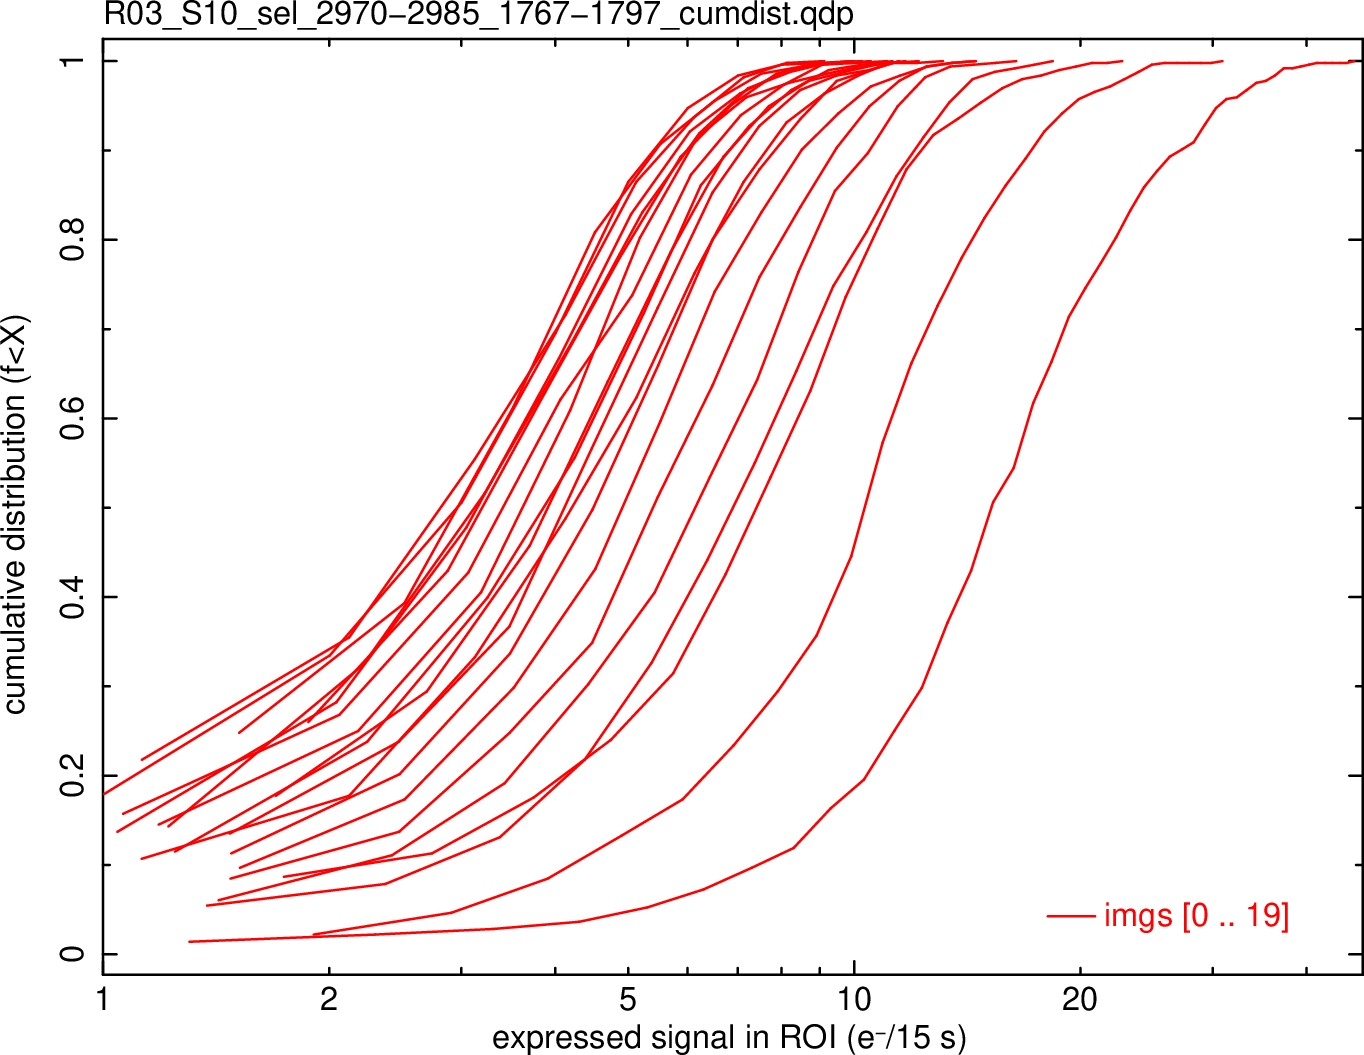
\includegraphics[width=\textwidth]{figures/phosphorescence-survey/phos_kinetics/R03_S10_sel_2970-2985_1767-1797_cumdist.png}    
\end{subfigure}
\hfil
\begin{subfigure}{0.45\textwidth}
  \centering
  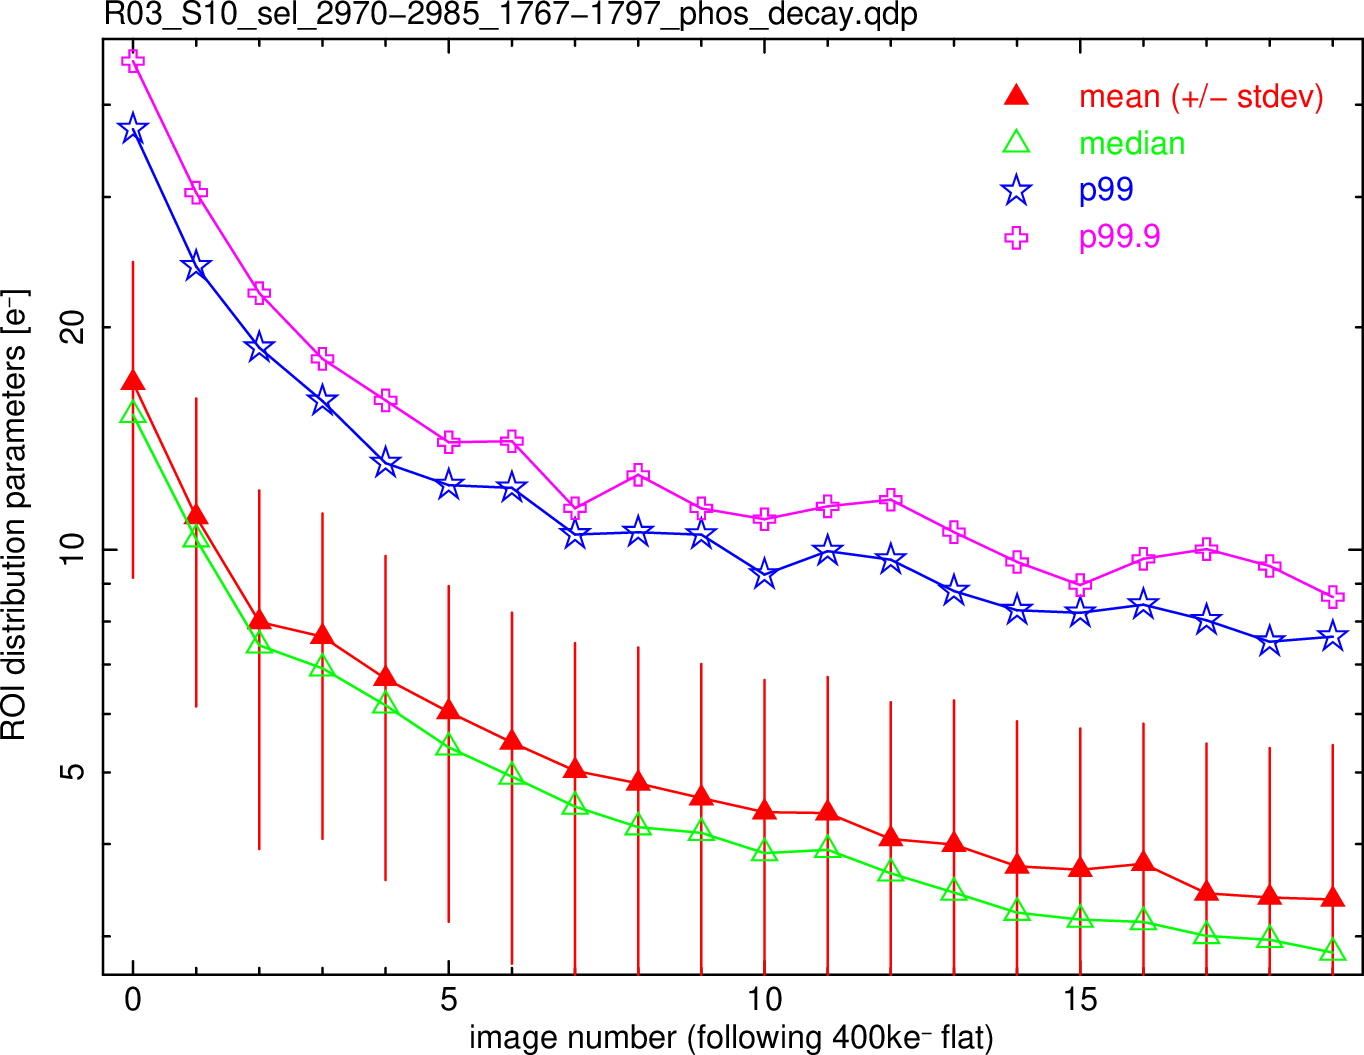
\includegraphics[width=\textwidth]{figures/phosphorescence-survey/phos_kinetics/R03_S10_sel_2970-2985_1767-1797_phos_decay.png}
\end{subfigure}
\newline
\begin{subfigure}{0.45\textwidth}    
  \centering
  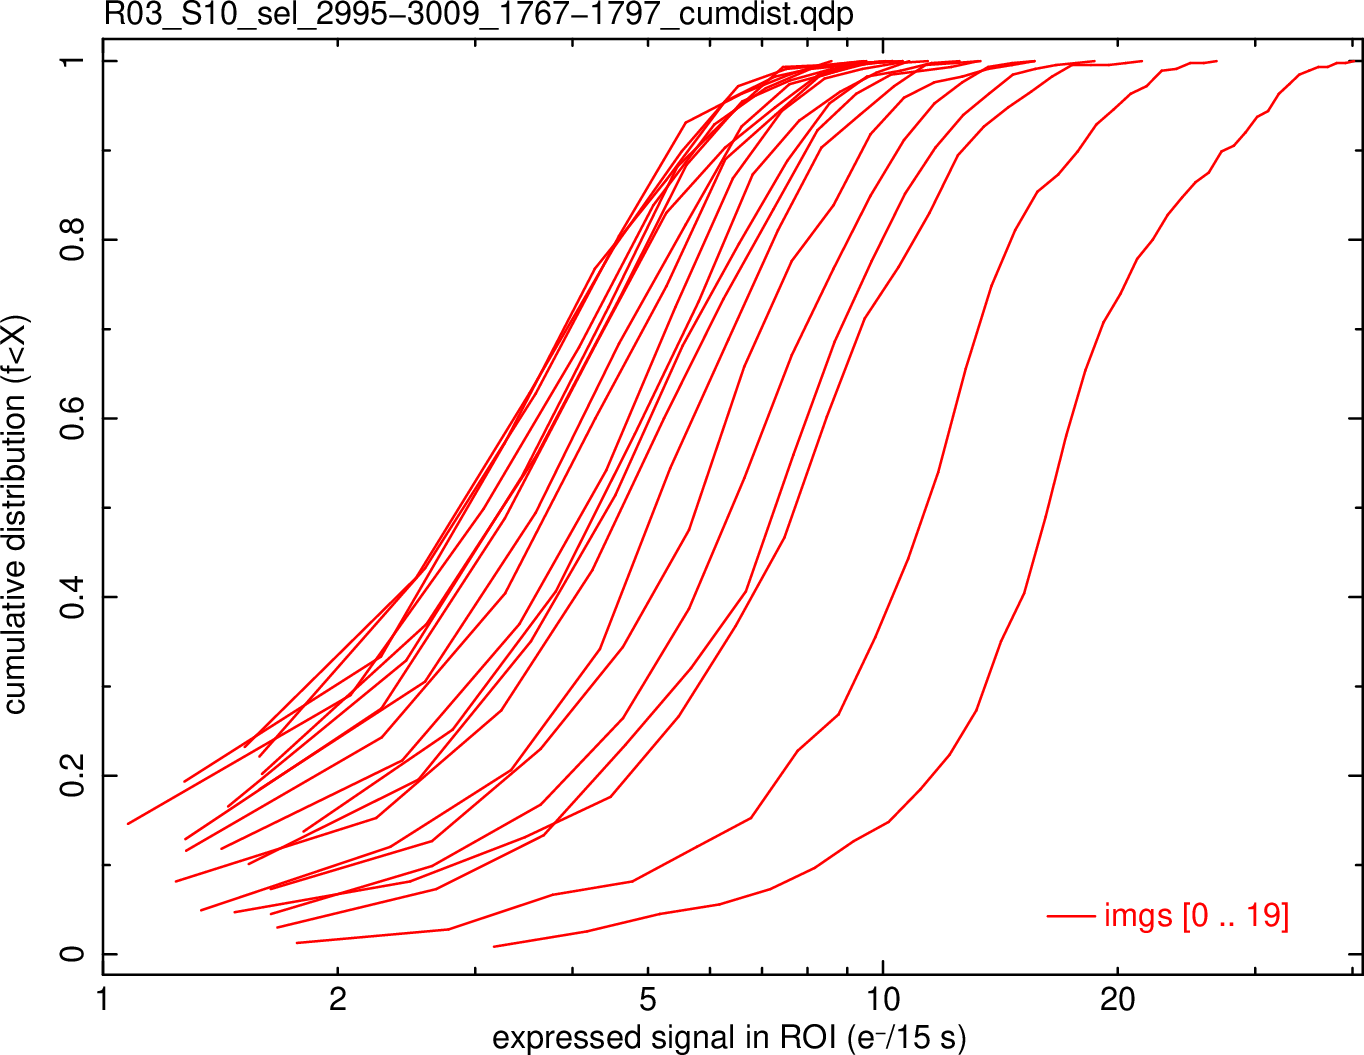
\includegraphics[width=\textwidth]{figures/phosphorescence-survey/phos_kinetics/R03_S10_sel_2995-3009_1767-1797_cumdist.png}    
\end{subfigure}
\hfil
\begin{subfigure}{0.45\textwidth}
  \centering
  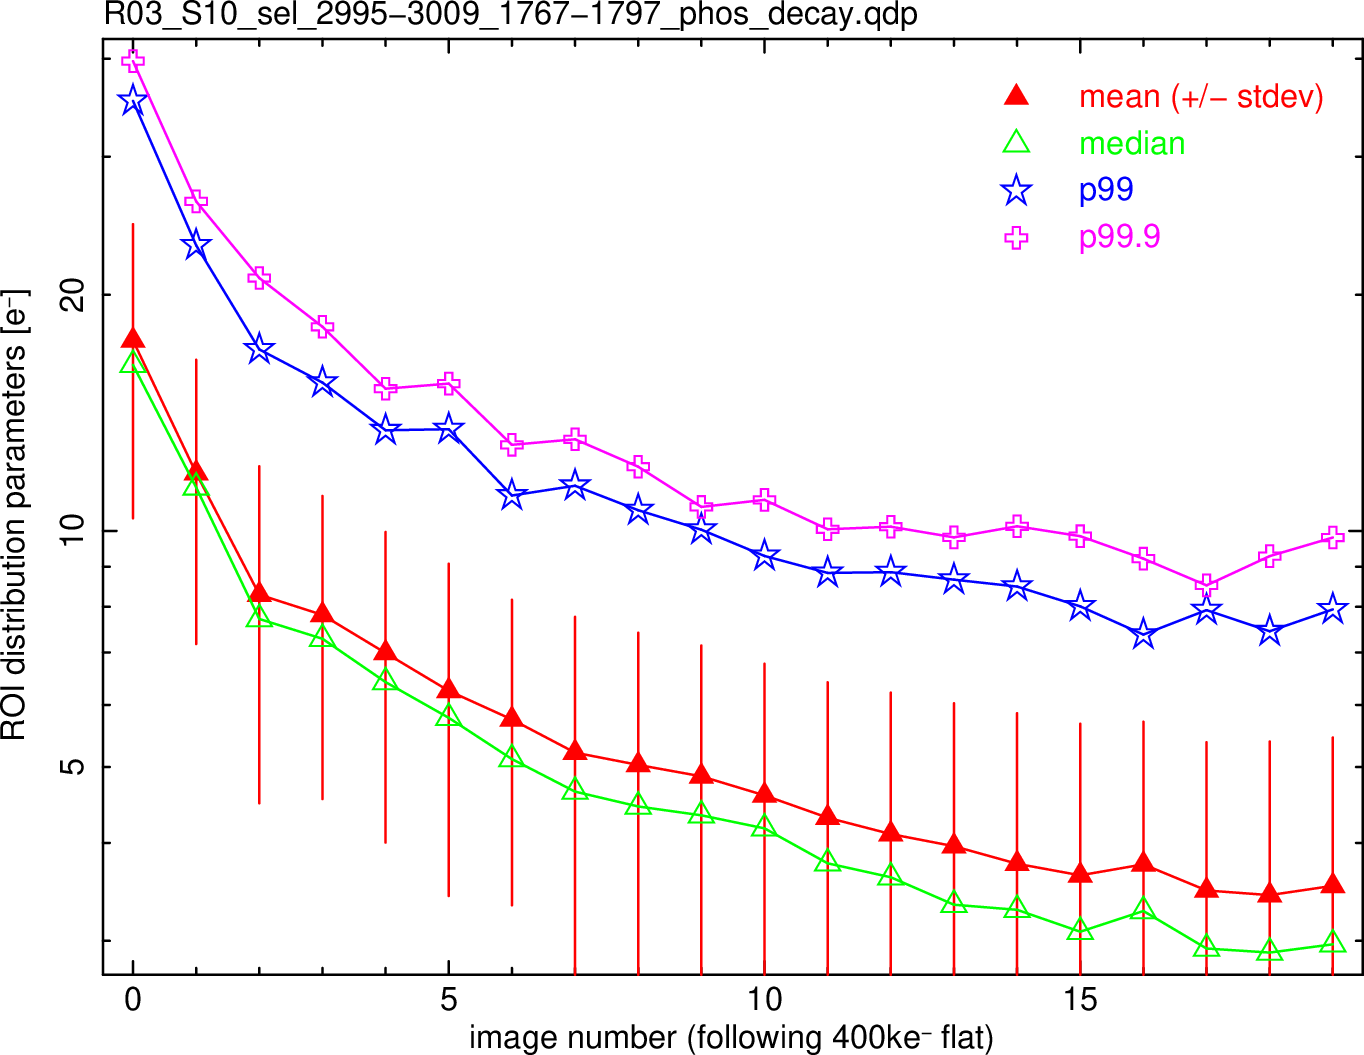
\includegraphics[width=\textwidth]{figures/phosphorescence-survey/phos_kinetics/R03_S10_sel_2995-3009_1767-1797_phos_decay.png}
\end{subfigure}
\newline
\caption{Kinetics for phosphorescence expression in ROIs of images for R03\_S10. These describe regions including or near the bright/focusing {\it vampire pixel} seen in Figs.~\ref{fig:phos:stains:R03S10}, \ref{subfig:phosresp_R03_S10} and \ref{subfig:hvb_on_R03_S10}.}
\label{fig:phos:kinetics:R03S10}
\end{figure}

\begin{figure}[!htbp]
\begin{subfigure}{0.45\textwidth}    
  \centering
  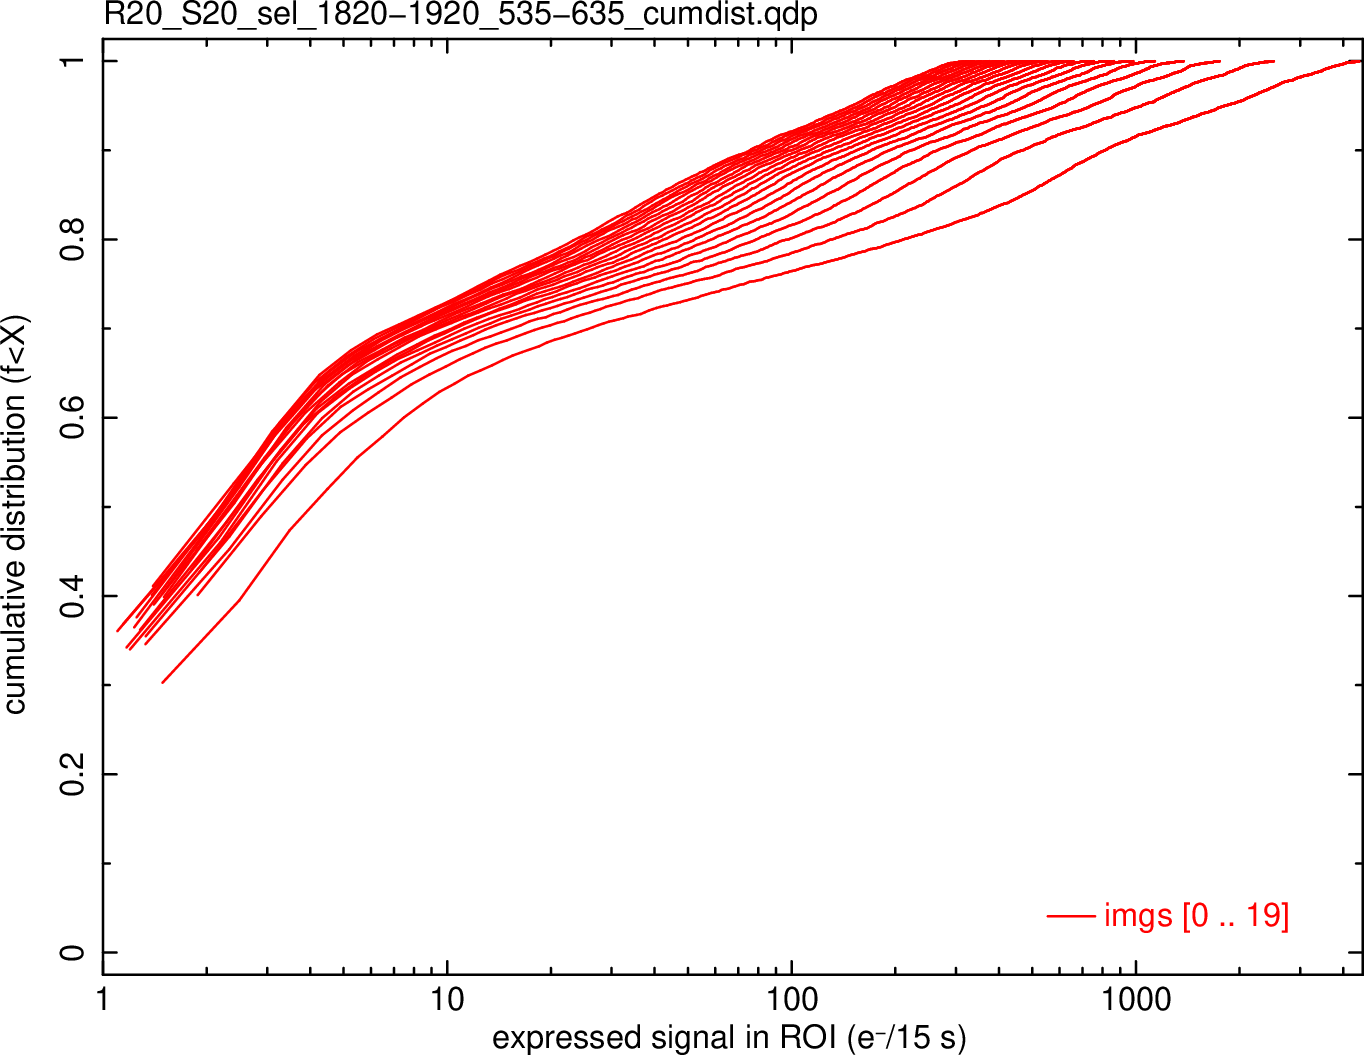
\includegraphics[width=\textwidth]{figures/phosphorescence-survey/phos_kinetics/R20_S20_sel_1820-1920_535-635_cumdist.png}    
\end{subfigure}
\hfil
\begin{subfigure}{0.45\textwidth}
  \centering
  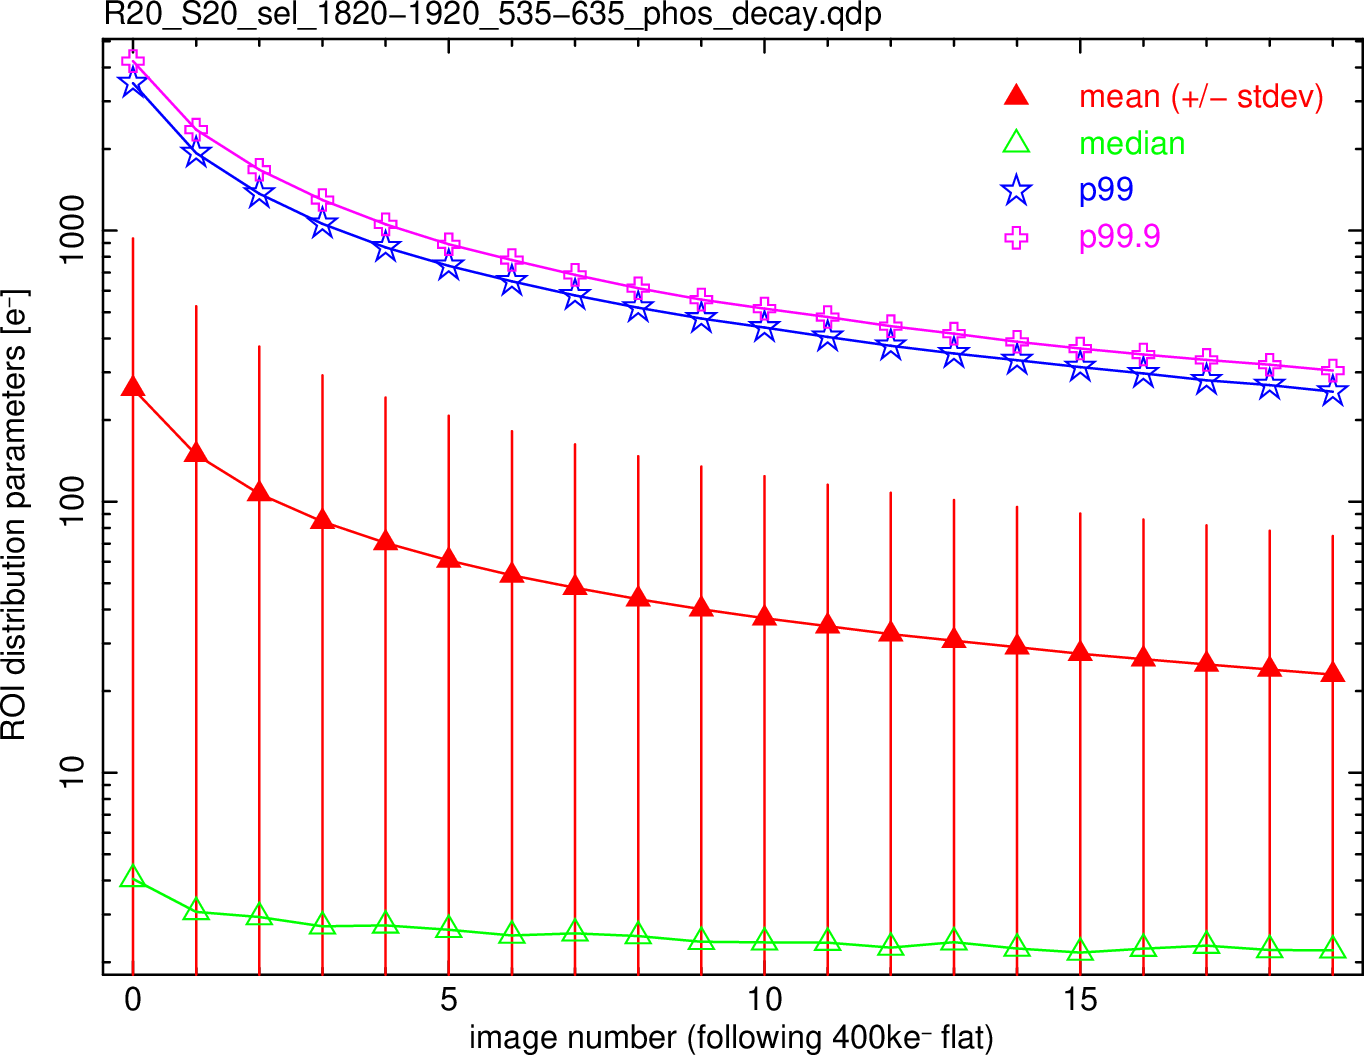
\includegraphics[width=\textwidth]{figures/phosphorescence-survey/phos_kinetics/R20_S20_sel_1820-1920_535-635_phos_decay.png}
\end{subfigure}
\newline
\caption{Kinetics for phosphorescence expression in ROIs of images for R20\_S20. These describe the prominent non-focusing {\it vampire pixel} seen in Figs.~\ref{subfig:phosresp_R20_S20} and \ref{subfig:hvb_on_R20_S20}.}
\label{fig:phos:kinetics:R20S20}
\end{figure}

\begin{figure}[!htbp]
\begin{subfigure}{0.45\textwidth}    
  \centering
  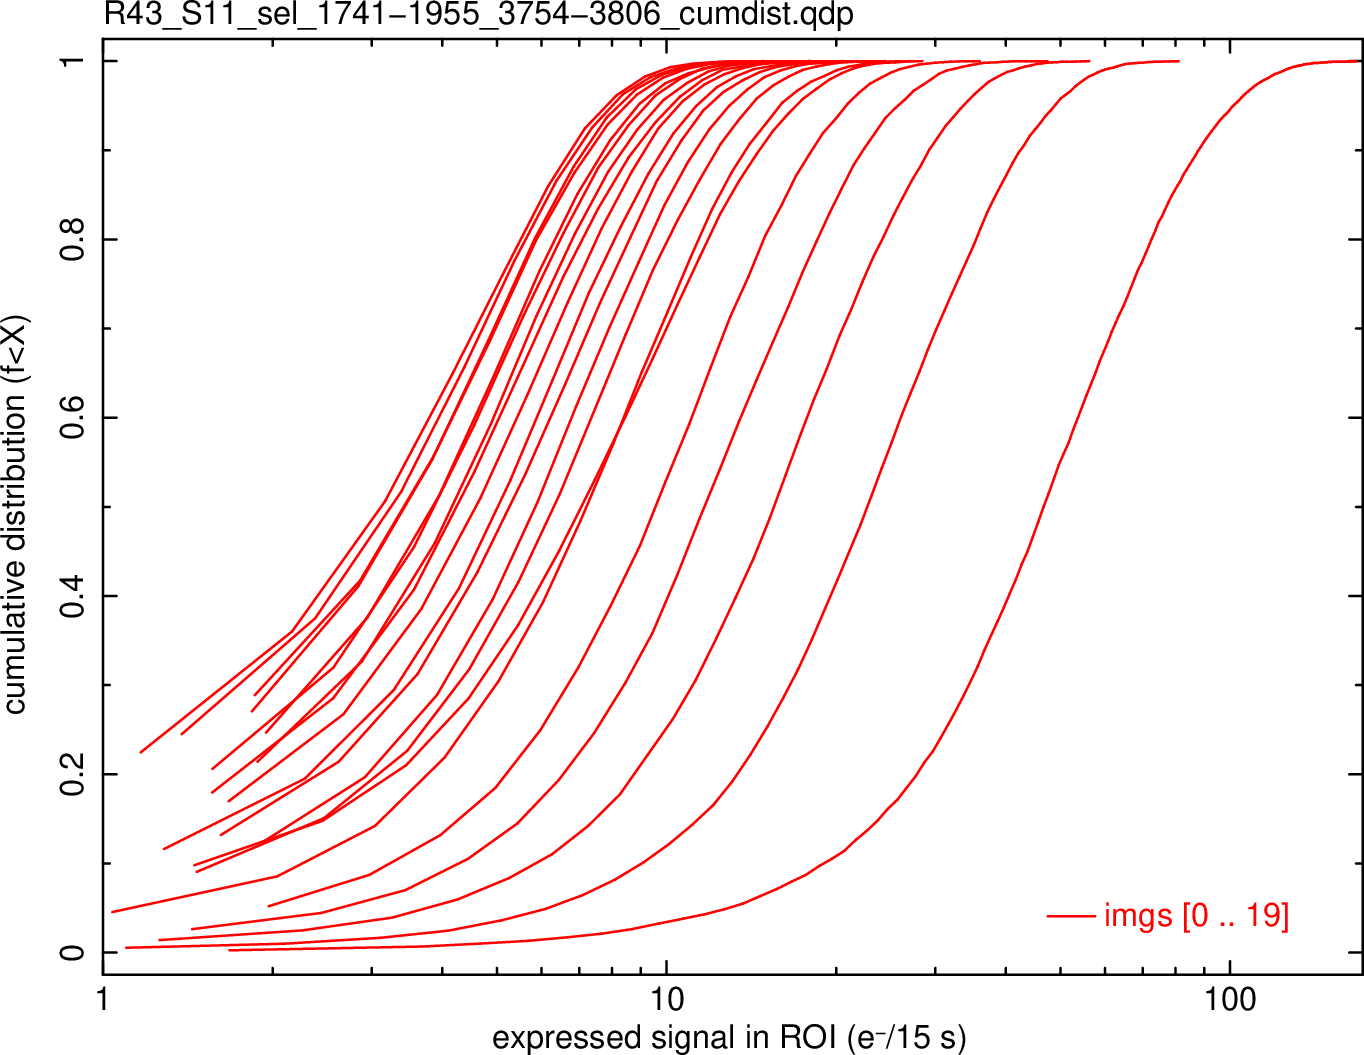
\includegraphics[width=\textwidth]{figures/phosphorescence-survey/phos_kinetics/R43_S11_sel_1741-1955_3754-3806_cumdist.png}    
\end{subfigure}
\hfil
\begin{subfigure}{0.45\textwidth}
  \centering
  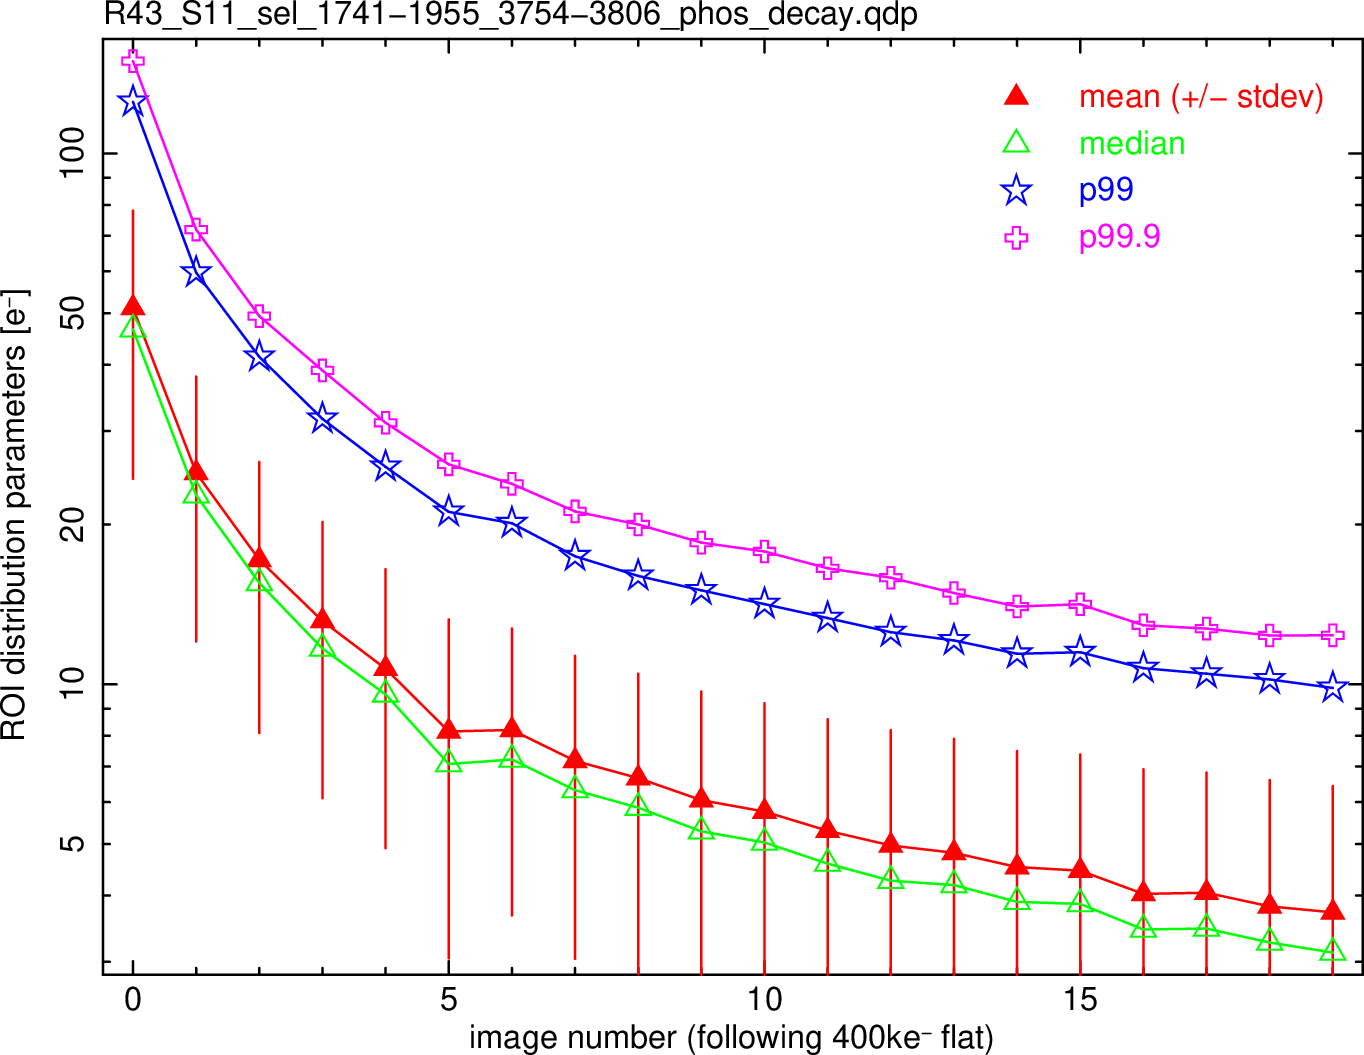
\includegraphics[width=\textwidth]{figures/phosphorescence-survey/phos_kinetics/R43_S11_sel_1741-1955_3754-3806_phos_decay.png}
\end{subfigure}
\newline
\begin{subfigure}{0.45\textwidth}    
  \centering
  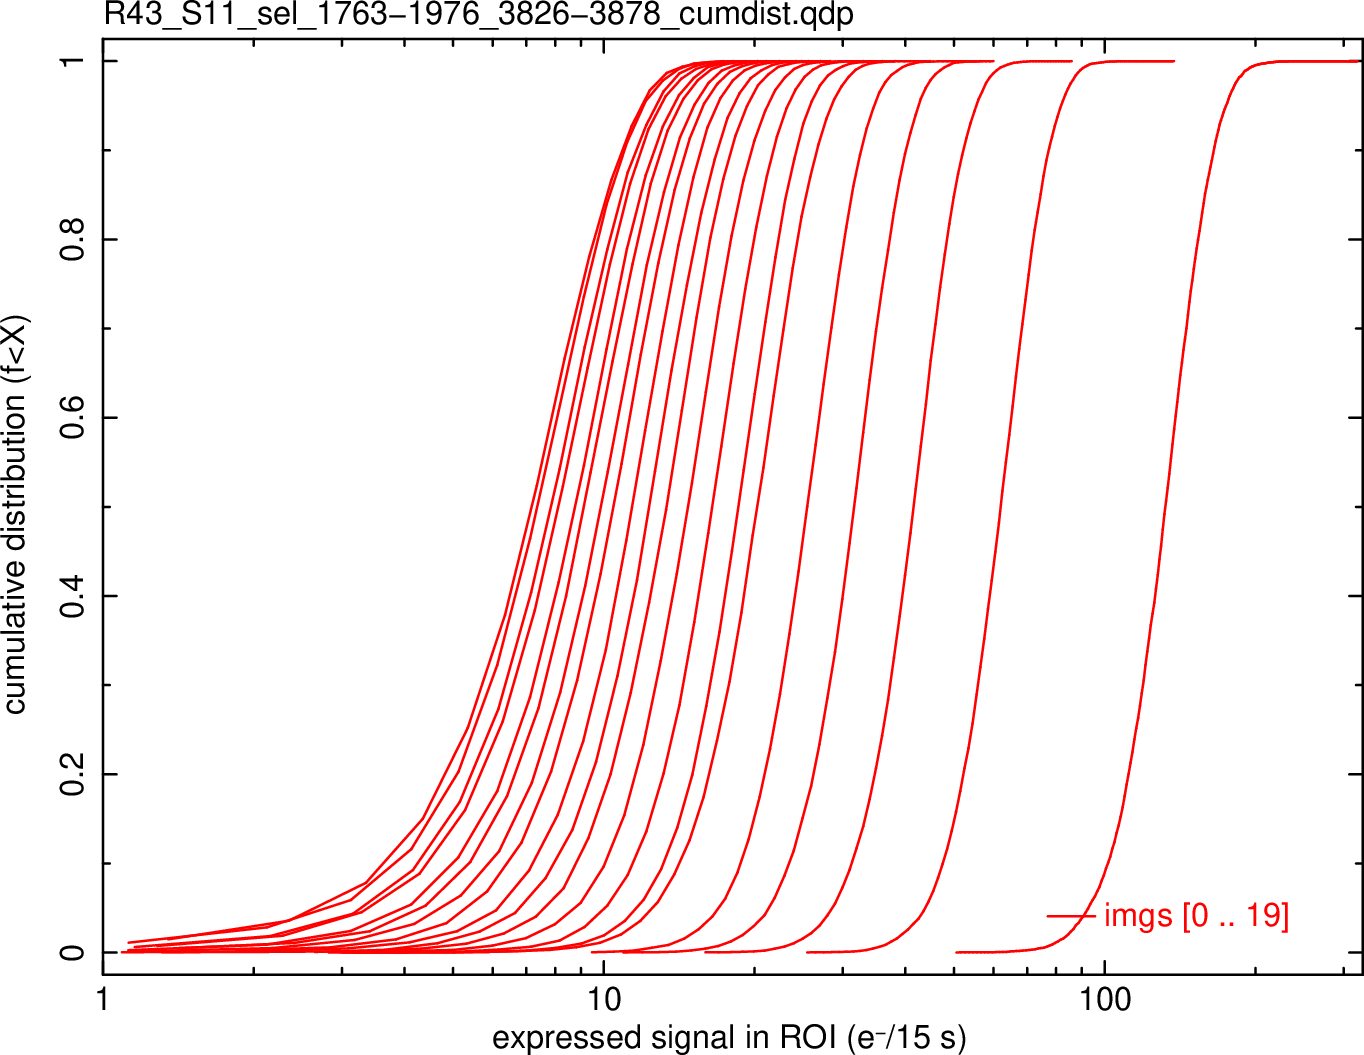
\includegraphics[width=\textwidth]{figures/phosphorescence-survey/phos_kinetics/R43_S11_sel_1763-1976_3826-3878_cumdist.png}    
\end{subfigure}
\hfil
\begin{subfigure}{0.45\textwidth}
  \centering
  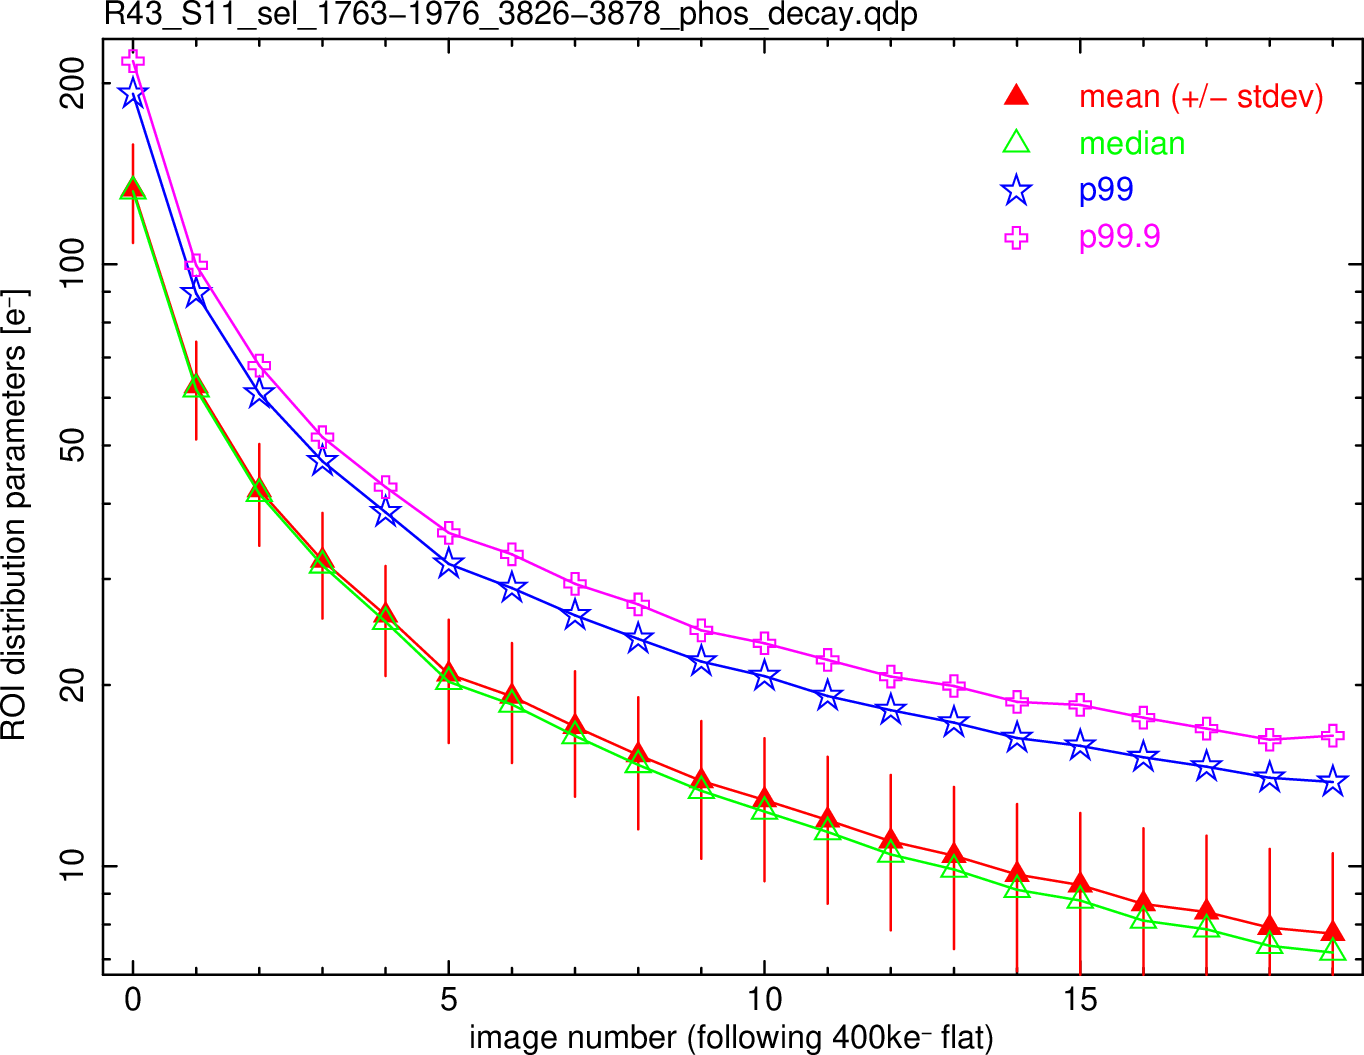
\includegraphics[width=\textwidth]{figures/phosphorescence-survey/phos_kinetics/R43_S11_sel_1763-1976_3826-3878_phos_decay.png}
\end{subfigure}
\newline
\begin{subfigure}{0.45\textwidth}    
  \centering
  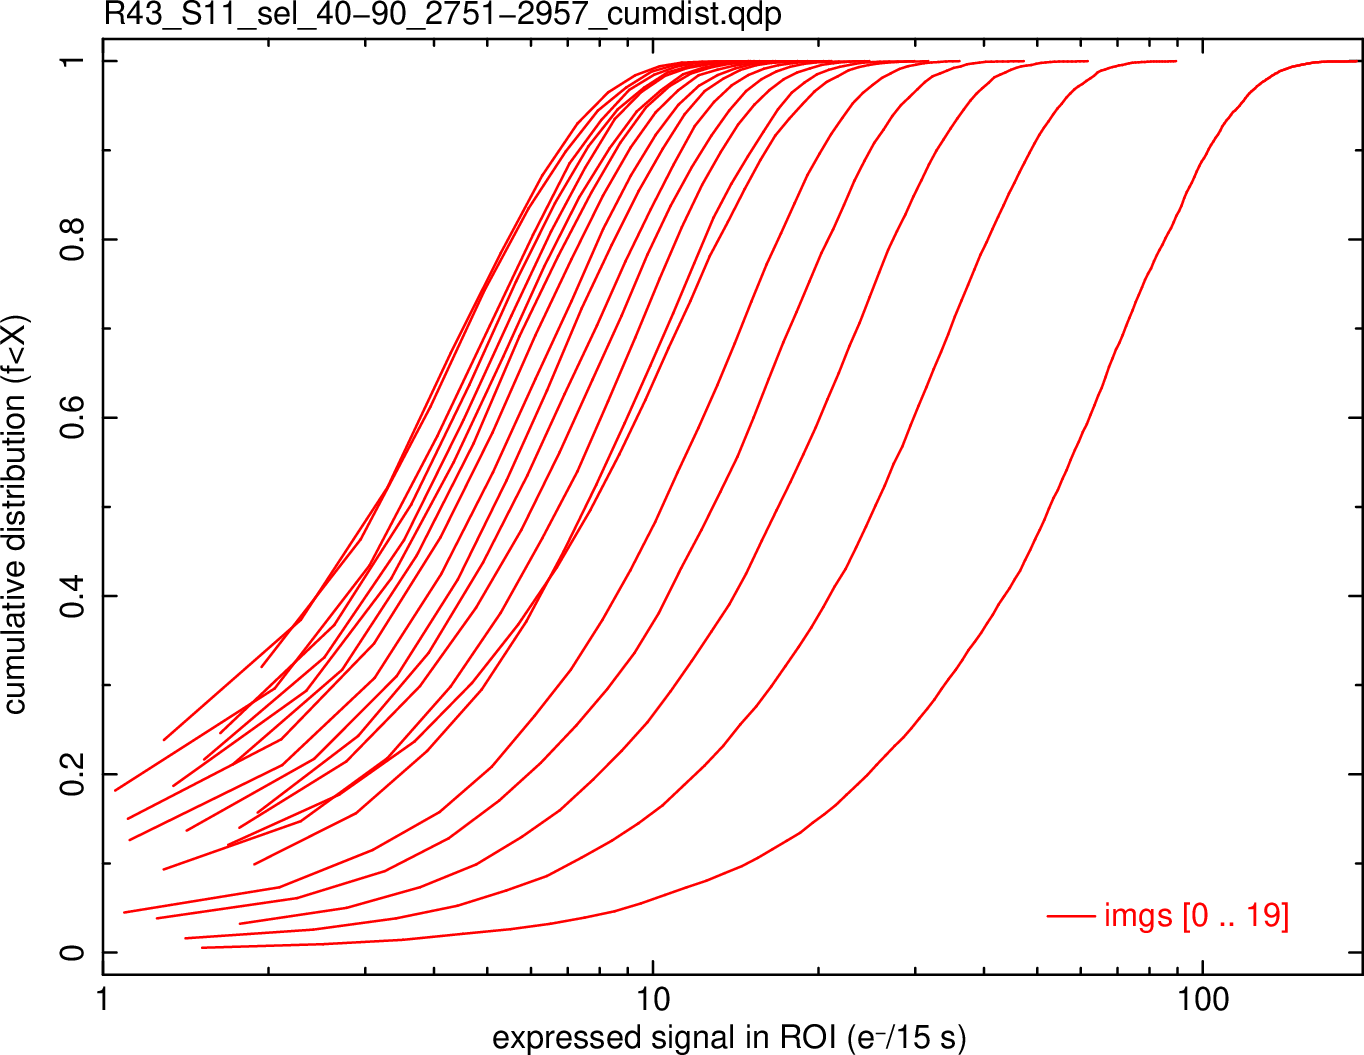
\includegraphics[width=\textwidth]{figures/phosphorescence-survey/phos_kinetics/R43_S11_sel_40-90_2751-2957_cumdist.png}    
\end{subfigure}
\hfil
\begin{subfigure}{0.45\textwidth}
  \centering
  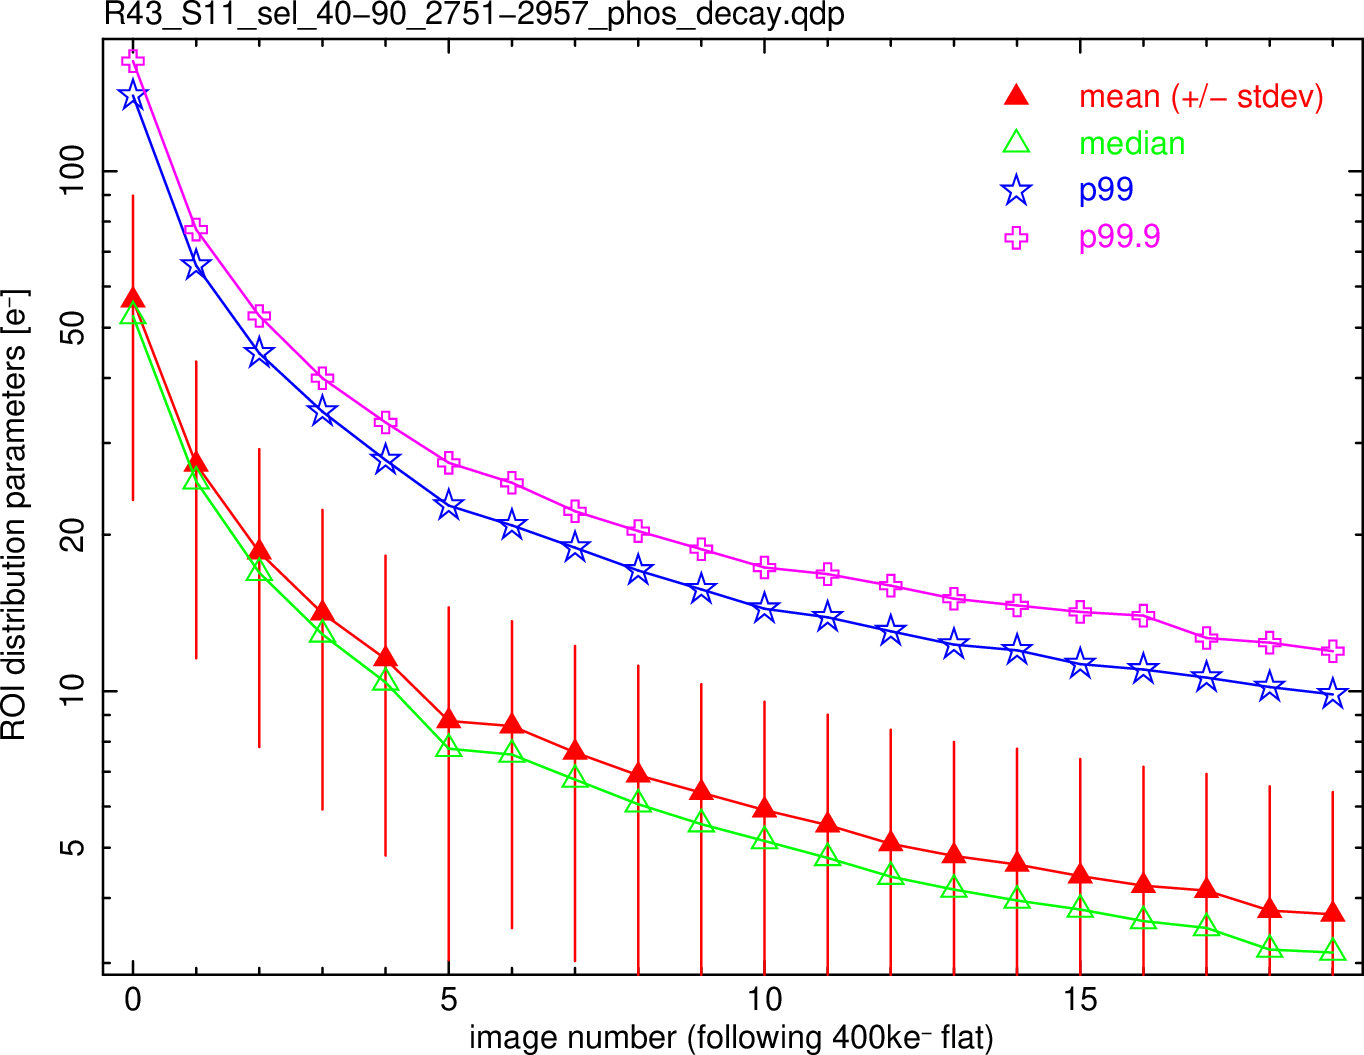
\includegraphics[width=\textwidth]{figures/phosphorescence-survey/phos_kinetics/R43_S11_sel_40-90_2751-2957_phos_decay.png}
\end{subfigure}
\newline
\caption{Kinetics for phosphorescence expression in ROIs of images for R43\_S11. These describe bright, diffuse transient regions seen in Figs.~\ref{fig:phos:stains:R43S11} and \ref{subfig:hvb_on_R43_S11}, which apparently turn off completely when the HV Bias is {\it off}.}
\label{fig:phos:kinetics:R43S11}
\end{figure}

\begin{figure}[!htbp]
\begin{subfigure}{0.45\textwidth}    
  \centering
  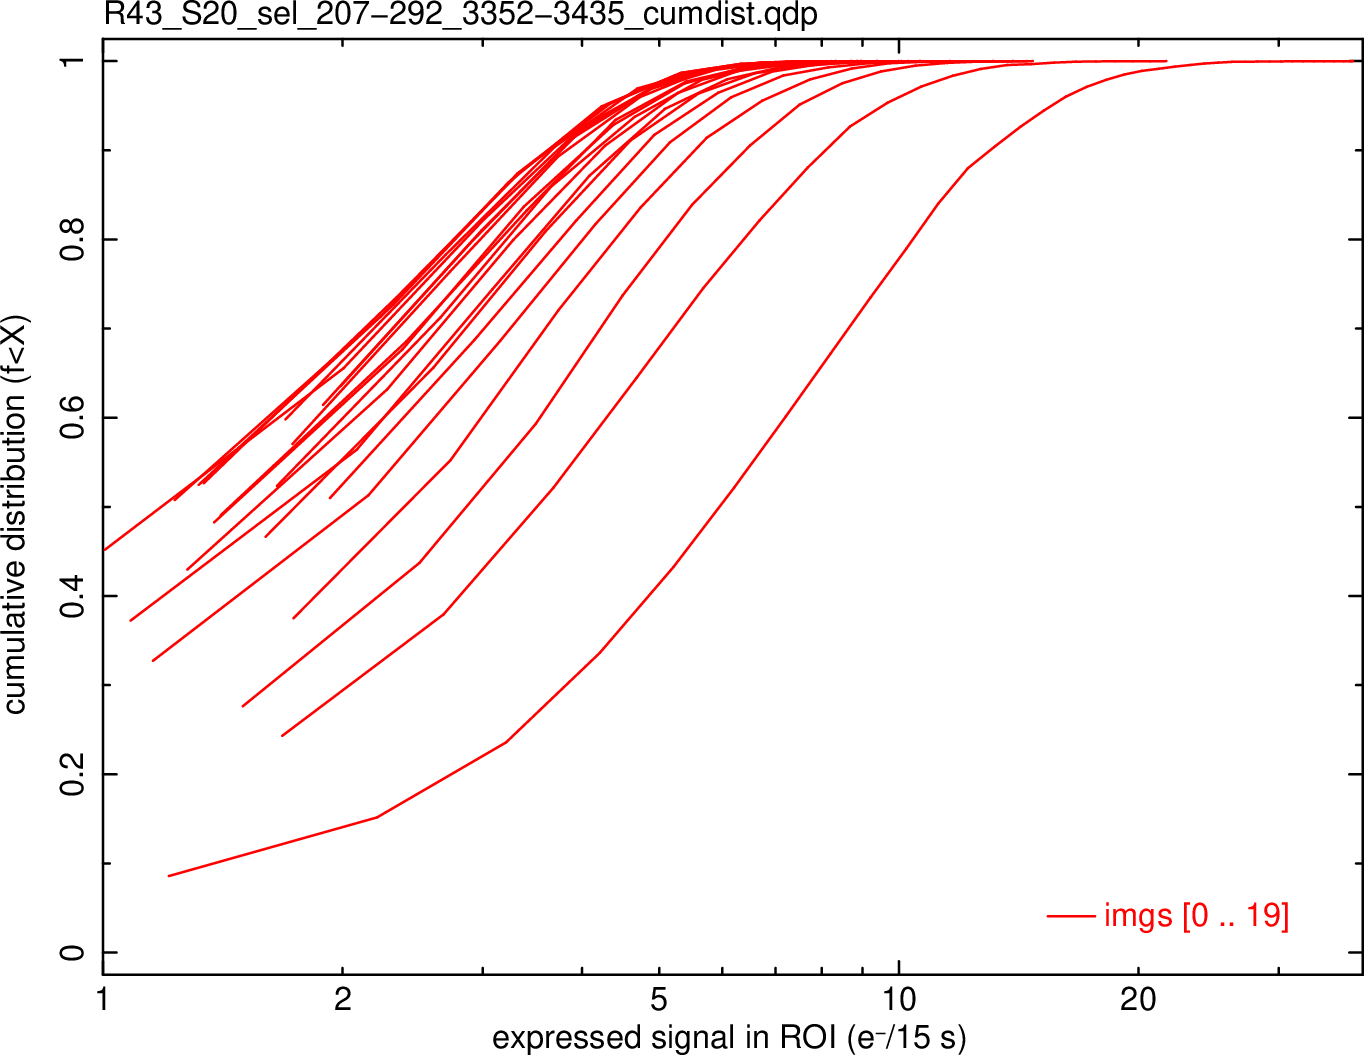
\includegraphics[width=\textwidth]{figures/phosphorescence-survey/phos_kinetics/R43_S20_sel_207-292_3352-3435_cumdist.png}    
\end{subfigure}
\hfil
\begin{subfigure}{0.45\textwidth}
  \centering
  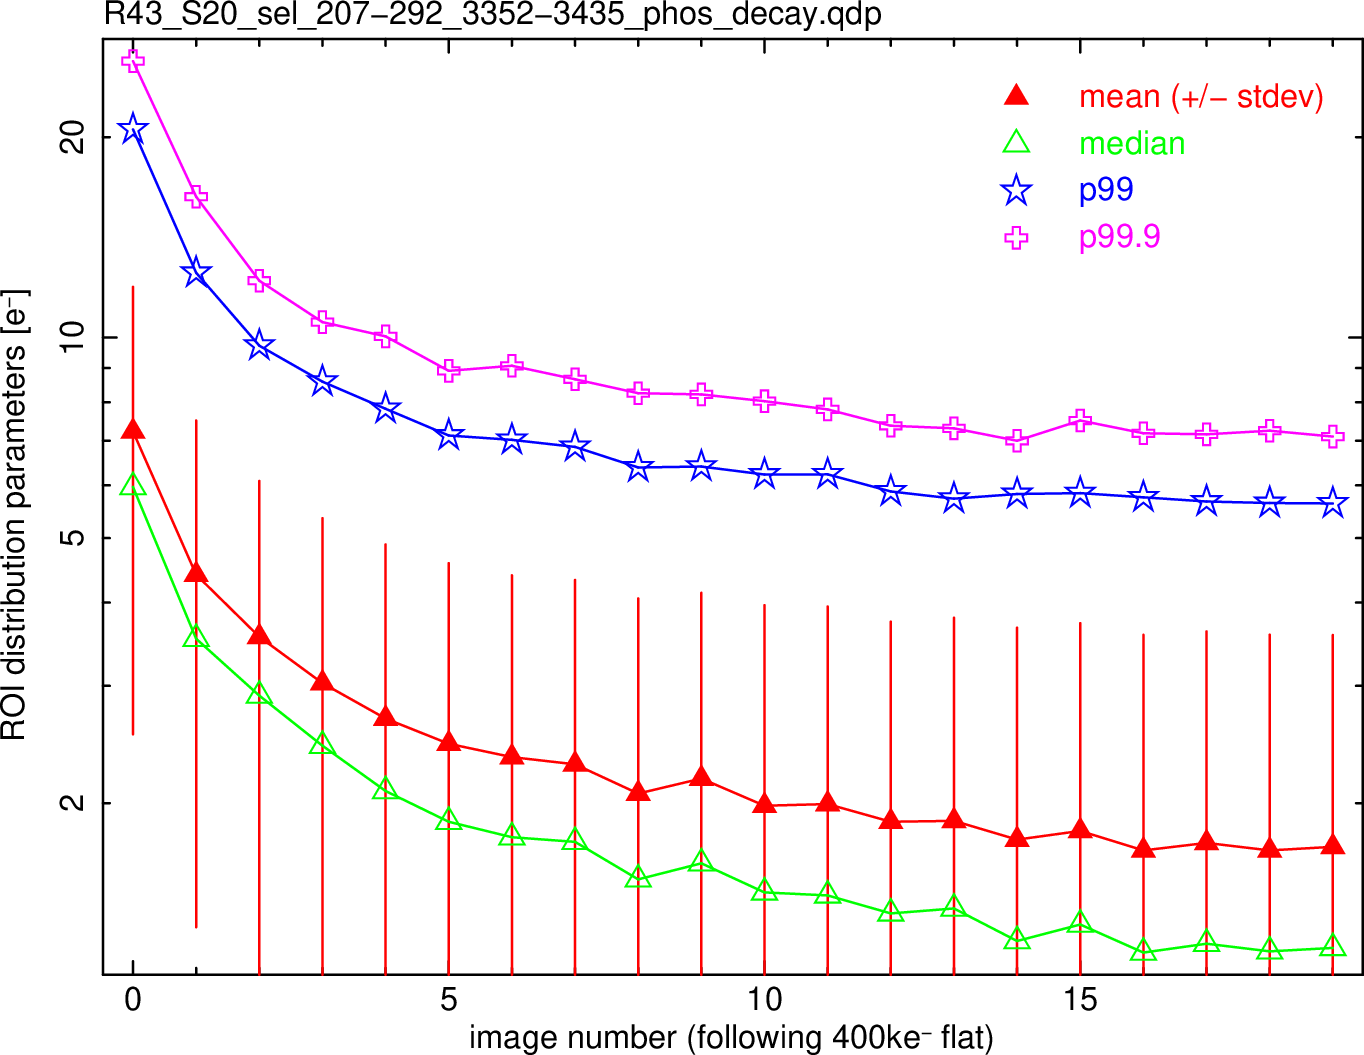
\includegraphics[width=\textwidth]{figures/phosphorescence-survey/phos_kinetics/R43_S20_sel_207-292_3352-3435_phos_decay.png}
\end{subfigure}
\newline
\begin{subfigure}{0.45\textwidth}    
  \centering
  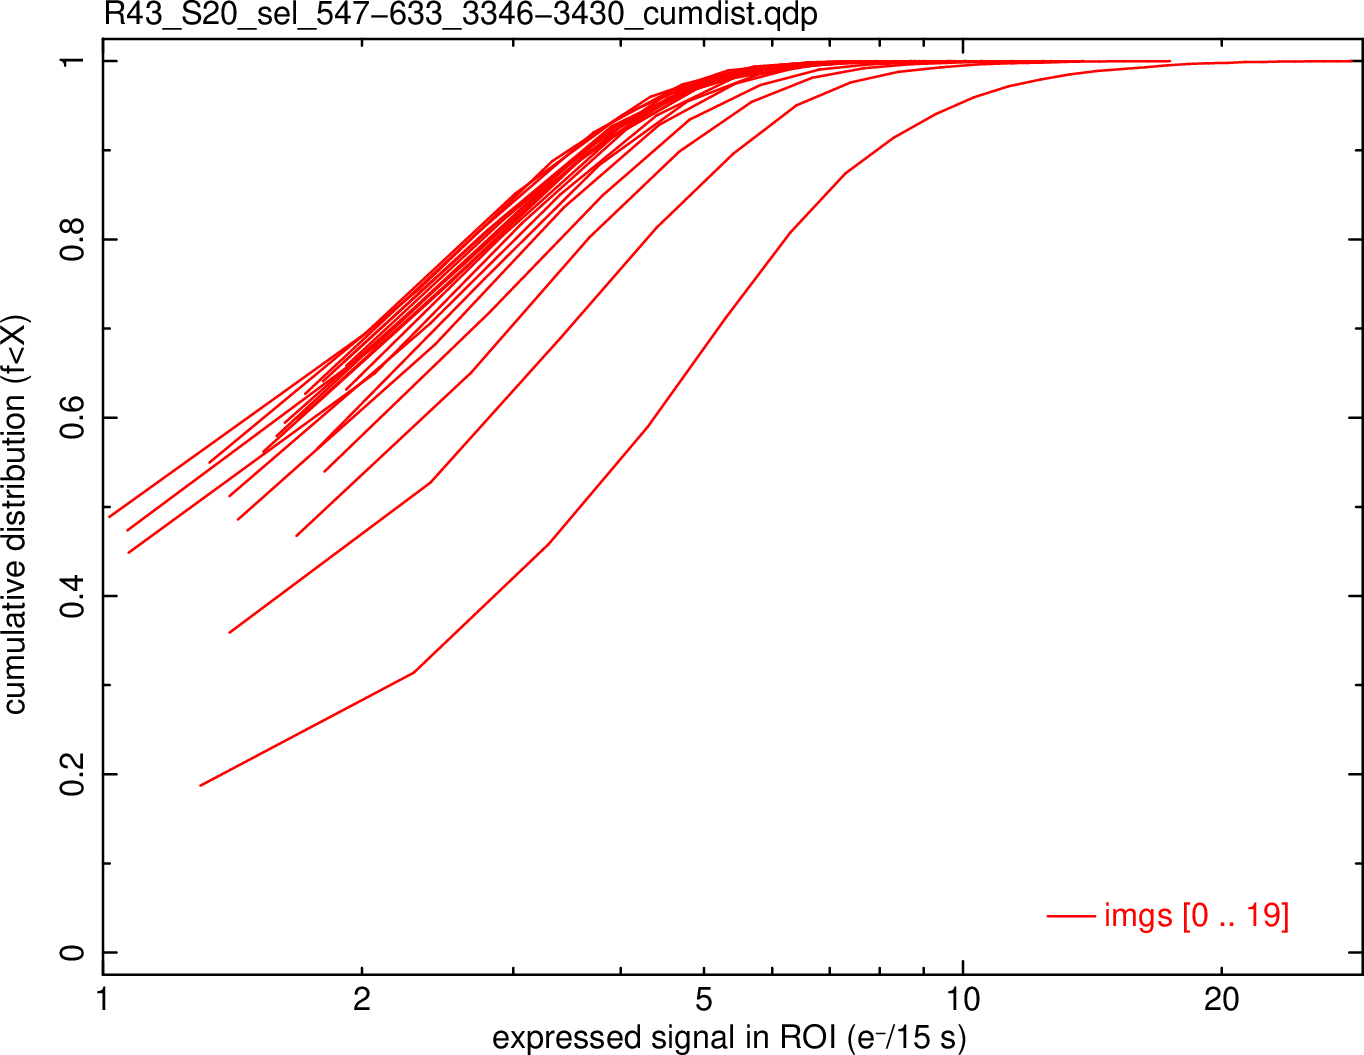
\includegraphics[width=\textwidth]{figures/phosphorescence-survey/phos_kinetics/R43_S20_sel_547-633_3346-3430_cumdist.png}    
\end{subfigure}
\hfil
\begin{subfigure}{0.45\textwidth}
  \centering
  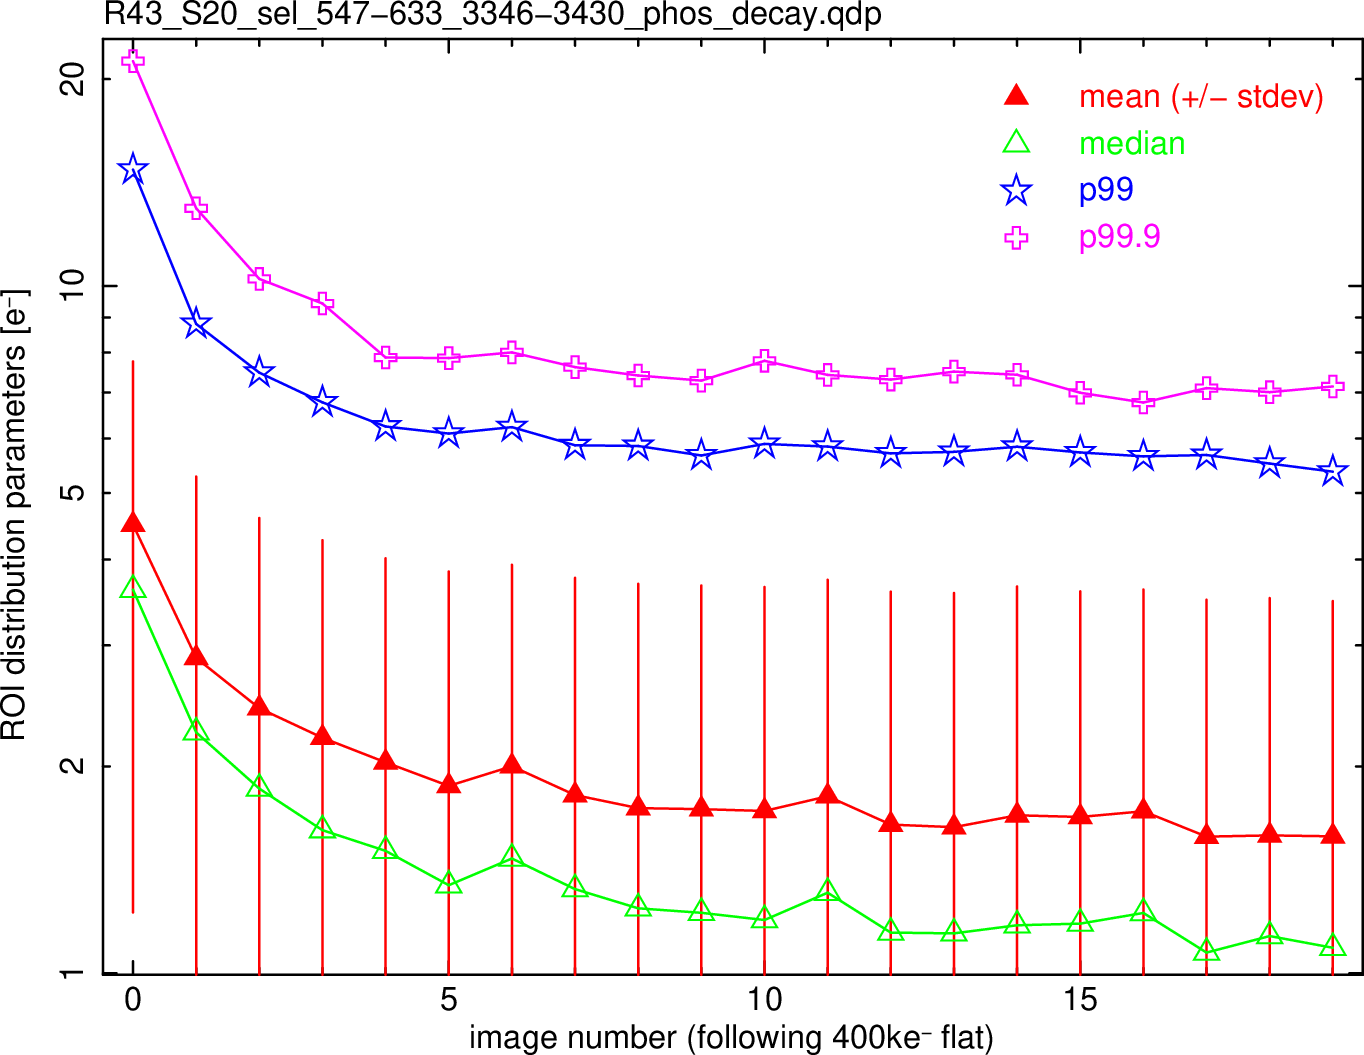
\includegraphics[width=\textwidth]{figures/phosphorescence-survey/phos_kinetics/R43_S20_sel_547-633_3346-3430_phos_decay.png}
\end{subfigure}
\newline
\begin{subfigure}{0.45\textwidth}    
  \centering
  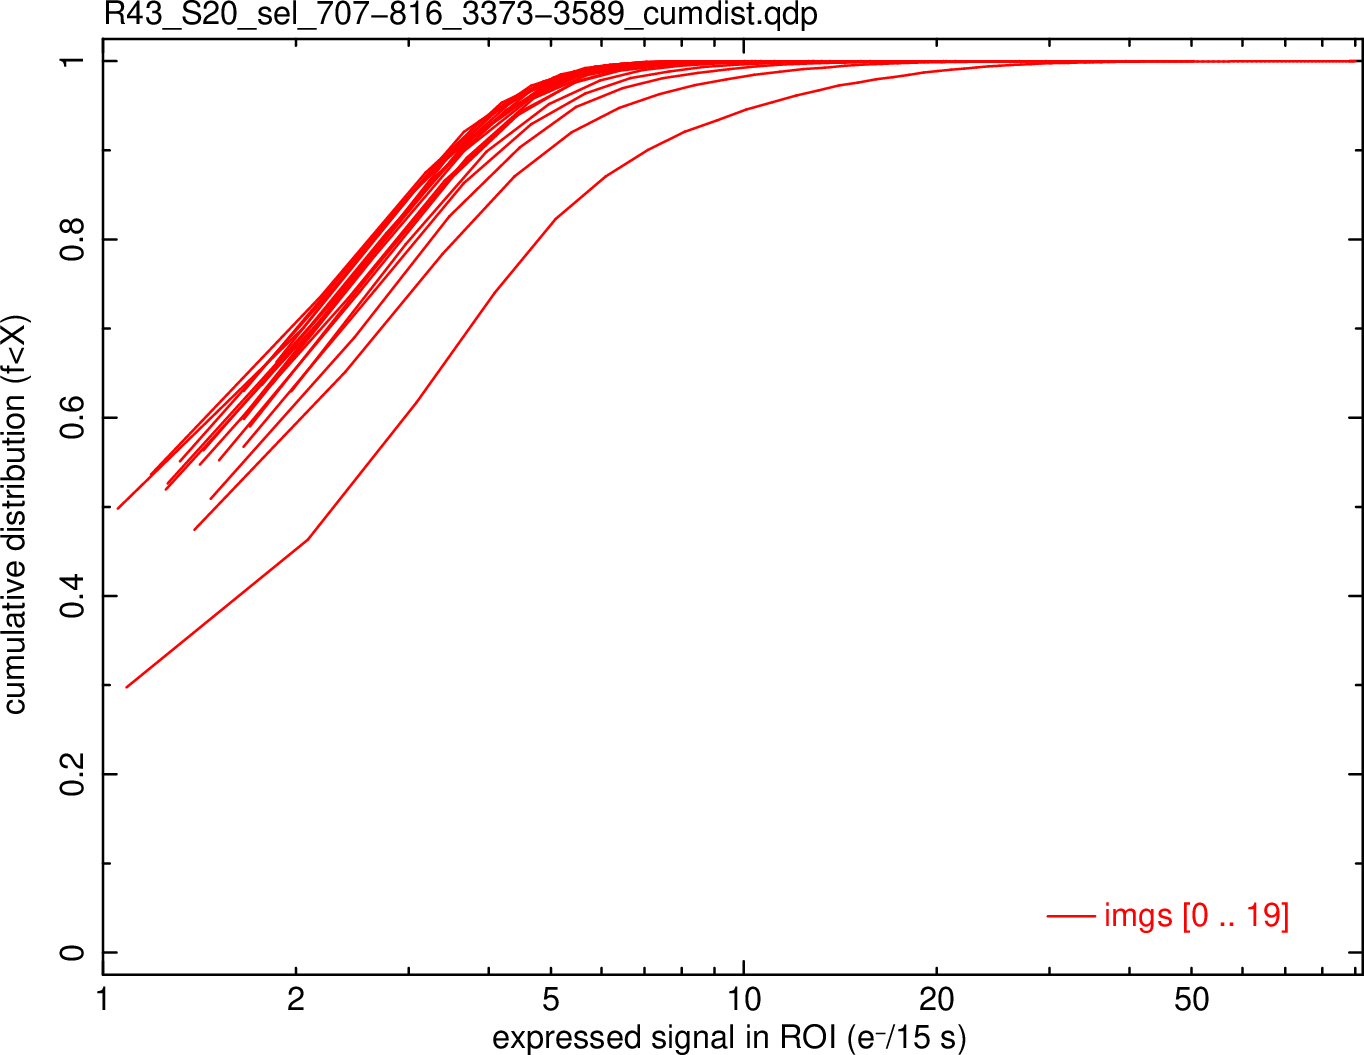
\includegraphics[width=\textwidth]{figures/phosphorescence-survey/phos_kinetics/R43_S20_sel_707-816_3373-3589_cumdist.png}    
\end{subfigure}
\hfil
\begin{subfigure}{0.45\textwidth}
  \centering
  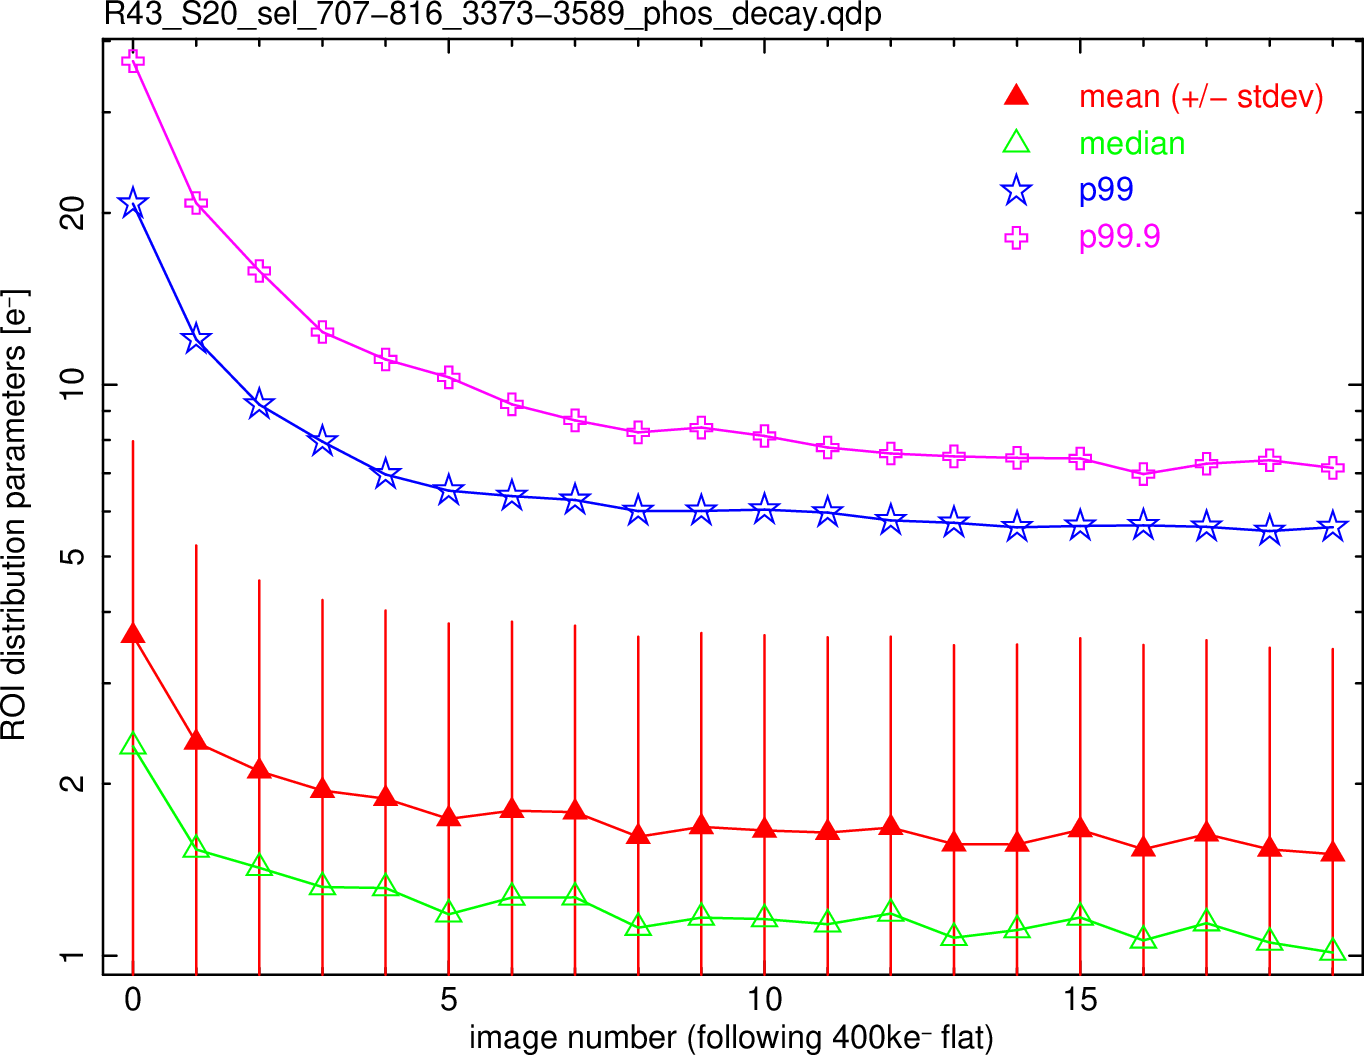
\includegraphics[width=\textwidth]{figures/phosphorescence-survey/phos_kinetics/R43_S20_sel_707-816_3373-3589_phos_decay.png}
\end{subfigure}
\newline
\caption{Kinetics for phosphorescence expression in ROIs of images for R43\_S20. These include some of the the highly structured {\it snowflake-like} transient regions seen in Figs.~\ref{subfig:hvb_on_R43_S20} and \ref{fig:phos:stains:R43S20}.}
\label{fig:phos:kinetics:R43S20}
\end{figure}
